\documentclass[11pt,a4paper]{report}

% ==================== Page Geometry ====================
\usepackage[margin=1in]{geometry}

% ==================== Fonts & Encoding ====================
\usepackage[T1]{fontenc}
\usepackage[utf8]{inputenc}
\usepackage{lmodern}

% ==================== Math ====================
\usepackage{amsmath,amssymb,amsthm}
\numberwithin{equation}{section}

% ==================== Theorems ====================
\theoremstyle{definition}
\newtheorem{definition}{Definition}[section]
\newtheorem{theorem}{Theorem}[section]
\newtheorem{proposition}{Proposition}[section]
\newtheorem{example}{Example}[section]
\theoremstyle{remark}
\newtheorem{remark}{Remark}[section]

% ==================== Figures & Tables ====================
\usepackage{graphicx}
\usepackage{booktabs}
\usepackage{tabularx}

% ==================== Ti\textit{k}Z ====================
\usepackage{tikz}
\usetikzlibrary{calc,positioning,shapes.geometric,arrows.meta,decorations.pathreplacing}

% ==================== Algorithm Pseudocode ====================
\usepackage{algorithm}
\usepackage{algpseudocode}

% ==================== Code Listings ====================
\usepackage{minted}
\setminted{
    fontsize=\small,
    linenos,
    numbersep=5pt,
    frame=lines,
    framesep=2mm,
    breaklines,
    breakanywhere,
    tabsize=4
}

% ==================== Hyperlinks ====================
\usepackage{hyperref}
\hypersetup{
    colorlinks=true,
    linkcolor=blue!60!black,
    citecolor=blue!60!black,
    urlcolor=blue!60!black
}

% ==================== Utilities ====================
\usepackage{xcolor}
\usepackage{setspace}
\usepackage{titlesec}
\usepackage{fancyvrb}

% Section title spacing
\titlespacing*{\chapter}{0pt}{0pt}{20pt}
\titlespacing*{\section}{0pt}{12pt plus 4pt minus 2pt}{6pt plus 2pt minus 1pt}
\titlespacing*{\subsection}{0pt}{10pt plus 3pt minus 2pt}{4pt plus 2pt minus 1pt}

% Line spacing
\onehalfspacing

% ==================== Document Info ====================
\title{\vspace{-2em}\Huge\bfseries Feature-Based Face Morphing: A Step-by-Step Tutorial}
\author{\Large Hongbo Meng}
\date{\large \today}

% ==================== Begin Document ====================
\begin{document}

\maketitle

\thispagestyle{empty}
\newpage

\begin{abstract}
This tutorial provides a comprehensive, step-by-step explanation of the feature-based face morphing
algorithm --- a technique that produces natural-looking averaged faces by aligning facial features
before blending. We cover every component in depth: facial landmark detection, affine transformations,
barycentric coordinates, Delaunay triangulation, piecewise affine warping, and alpha blending.
Each section includes mathematical derivations, visual illustrations using Ti\textit{k}Z diagrams,
and a complete Python implementation supporting both \texttt{dlib} and \texttt{MediaPipe} backends.
By the end of this tutorial, you will understand not only \emph{how} face morphing works, but
\emph{why} each design choice matters.
\end{abstract}

\newpage
\tableofcontents
\newpage

% ==================== Sections ====================

\section{Introduction}

When two people stand side by side and we ask what they would look like as a single person, our
imagination instinctively tries to merge their features. We picture the eye shape of one person
combined with the jawline of the other, the nose of this person blended with the smile of that
person. This intuitive notion of ``averaging'' faces is precisely what computational face
averaging attempts to formalize. Yet what feels natural to the human brain becomes a surprisingly
rich algorithmic challenge when we ask a computer to perform this task.

This tutorial walks through every step of building a \emph{feature-based} face morphing system ---
one that produces convincing, natural-looking results by aligning facial geometry before blending
pixel values. Along the way, we will encounter concepts from computer vision, computational
geometry, linear algebra, and image processing. No single technique is particularly difficult, but
the way they fit together is elegant and instructive.


\subsection{What Is Face Averaging and Face Morphing?}

At its core, \emph{face averaging} answers a simple question: given two or more photographs of
different people's faces, can we produce a single image that represents their collective
appearance? The output should look like a plausible human face --- not a superimposed jumble, not
a half-and-half split, but a coherent image that could have been captured by a camera.

It helps to distinguish two closely related terms that are often used interchangeably but carry
subtly different meanings.

\begin{description}
    \item[Face Averaging] refers to the static problem of computing a single representative face
    from a set of input faces. The word ``average'' here is used in the everyday sense: we want
    something that embodies characteristics of all inputs. A common technique is to compute the
    mean of corresponding pixel values across aligned images, but as we will see shortly, a raw
    pixel average produces unsatisfactory results without careful geometric alignment first.

    \item[Face Morphing] refers to the dynamic, time-varying process of creating a smooth
    \emph{transition} from one face to another. A morph is a sequence of frames in which the
    first frame is face A, the last frame is face B, and every intermediate frame shows a
    progressively larger contribution from B and a smaller contribution from A. Face morphing
    is more general than face averaging because it requires producing not just one blended image
    but an entire continuous family of them, parameterized by a blending coefficient $\alpha \in
    [0, 1]$. When $\alpha = 0.5$, the morph frame is exactly an average of the two faces.
\end{description}

In this tutorial we focus primarily on the averaging problem ($\alpha = 0.5$ for two faces), but
everything we develop generalizes directly to morphing at arbitrary values of $\alpha$. Once we
know how to warp two faces into a common geometry and blend them at fifty percent, producing a
full morph sequence requires only a loop over different $\alpha$ values.

Formally, we can state the problem as follows.

\begin{definition}[Face Averaging]
Given $N$ input face images $I_1, I_2, \dots, I_N$, each containing a roughly frontal view of a
person's face, compute a single output image $I_{\text{avg}}$ that appears to be a plausible face
whose features are intermediate to those of all inputs. The output should satisfy two desirable
properties:
\begin{enumerate}
    \item \textbf{Geometric fidelity:} Facial features (eyes, nose, mouth, jawline) in
    $I_{\text{avg}}$ should have shapes and positions that are intermediate between the
    corresponding features in each $I_k$.
    \item \textbf{Photorealism:} $I_{\text{avg}}$ should look like a real photograph of a face,
    not an obvious composite or computer-generated image. There should be no visible seams,
    ghosting, or blurring artifacts caused by misalignment.
\end{enumerate}
\end{definition}

The distinction between these two properties is important. Geometric fidelity concerns
\emph{where} features are placed, while photorealism concerns \emph{how} they look once placed.
The difficulty of face averaging arises because these two concerns interact: even with
perfectly accurate pixel values, placing them at the wrong locations produces visible artifacts.
Conversely, even with perfect geometry, poor blending of color and texture yields unrealistic
results. Our algorithm must address both.


\subsection{Applications of Face Averaging and Morphing}

Face averaging and morphing are not merely academic curiosities. They appear in a wide variety of
real-world contexts, some beneficial and some concerning. Understanding the applications motivates
why we should care about producing high-quality results.


\subsubsection{Law Enforcement and Forensics}

One of the oldest and most socially valuable applications is in forensic imagery.
Investigating officers sometimes need to reconstruct what a missing person might look like after
years of absence, or to create a composite image from multiple partial descriptions.

\begin{itemize}
    \item \textbf{Age progression.} When a child has been missing for years, law enforcement
    agencies produce age-progressed images to show what the person might look like as an adult.
    While this typically involves more than simple averaging --- bone structure changes, skin
    texture evolves, hair recedes --- morphing techniques form a building block of the process.
    A sequence of morphed images at increasing $\alpha$ values can suggest how facial structure
    changes over time when combined with models of aging.

    \item \textbf{Composite sketches.} When multiple witnesses describe a suspect, their
    descriptions may differ. Averaging the facial features described by independent witnesses
    can produce a composite that captures the common elements while smoothing out inconsistencies
    in any single account.

    \item \textbf{Identifying unknown individuals.} In cases where only degraded or partial
    facial images are available, morphing can be used to enhance recognition by combining
    information from multiple sources.
\end{itemize}


\subsubsection{Entertainment and Visual Effects}

The entertainment industry has long been a driving force behind morphing technology. Some of the
most memorable visual effects in cinema history rely on face morphing.

\begin{itemize}
    \item \textbf{Film and television effects.} The 1992 music video for Michael Jackson's
    ``Black or White'' featured a famous morphing sequence where one person's face smoothly
    transforms into another's. Such effects, once requiring expensive proprietary hardware, can
    now be produced on a laptop using the algorithms described in this tutorial.

    \item \textbf{Celebrity morphs and deepfake precursors.} Interactive websites and applications
    that let users morph their own face with a celebrity's are perennially popular. While modern
    deepfake technology has largely moved to neural-network-based approaches, the traditional
    feature-based morphing techniques we study here remain the foundation on which much of this
    work is built.

    \item \textbf{Character design.} In animation and video game development, artists sometimes
    average multiple source faces to create a new character whose appearance feels familiar yet
    distinctive. Averages of many faces tend to produce unusually attractive results --- a
    phenomenon we will discuss below --- making this a useful tool for character design.
\end{itemize}


\subsubsection{Cognitive Science and Psychology}

Perhaps the most scientifically surprising application of face averaging comes from the study of
human face perception. In 1878, Francis Galton --- a pioneer of statistics --- had an idea that
turned out to be remarkably prescient. He proposed that by superimposing multiple photographic
portraits, one could produce a ``composite photograph'' that represents the typical appearance of
a group.

Galton's original method was crude: he simply exposed a single photographic plate multiple times,
once for each person's portrait, with each exposure reduced in intensity. The resulting composite
turned out to be more attractive than essentially any of the individual faces that went into it.
This observation led to decades of research.

Modern confirmations of Galton's finding include:

\begin{itemize}
    \item \textbf{The ``averageness'' hypothesis.} Studies have repeatedly shown that composite
    faces --- whether created by photographic averaging or by computer morphing --- are rated as
    more attractive than individual faces. One explanation is that averageness signals genetic
    diversity and health. Another is that average faces are easier for the visual system to
    process (a ``processing fluency'' account).

    \item \textbf{Prototype formation.} Human brains appear to form prototype representations of
    faces automatically. When we see many faces of a particular demographic group, our visual
    system constructs an implicit ``average'' of those faces, which then becomes the baseline
    against which individual faces are compared. Morphing experiments allow researchers to probe
    this process by presenting controlled intermediate faces and measuring human responses.

    \item \textbf{Own-race bias.} People tend to be better at recognizing faces of their own racial
    or ethnic group than faces of other groups. Morphing studies have helped clarify whether this
    bias arises from perceptual familiarity (the prototype for other-race faces is less well
    developed) or from social factors.
\end{itemize}


\subsubsection{Biometric Security and Morphing Attacks}

On the more concerning side of applications, face morphing plays an important role in understanding
and attacking biometric security systems.

A \emph{morphing attack} on a face recognition system works as follows. An attacker creates a
morphed image that combines their own face with the face of an authorized person (the ``target'').
Because the morph contains features of both individuals, it may be accepted by the enrollment
system as belonging to the authorized person. Once the morphed image is enrolled in the database,
the attacker can then authenticate using their \emph{own} face, because the system has learned to
associate features of the attacker's face with the target's identity.

This attack vector is particularly dangerous in border control applications. If a forged passport
contains a morphed photograph of two different people, both people could potentially use that
single passport. The European Union's border control system has identified this as a significant
vulnerability, and research into morph detection has become a distinct subfield.

Understanding morphing attacks requires understanding morphing algorithms at a deep level. This is
why we study the full pipeline in this tutorial: the same techniques that produce beautiful
entertainment morphs also produce the morphs that can fool biometric systems, and knowing
how they work is essential for building defenses.


\subsection{The Naive Approach: Why Simple Pixel Averaging Fails}

Before developing a sophisticated algorithm, it is instructive to understand why the obvious
approach does not work. Consider the following naive strategy:

\begin{enumerate}
    \item Take two face images $I_1$ and $I_2$.
    \item Align them by identifying the centers of the eyes in each image and applying a global
    similarity transform (rotation, translation, and uniform scaling) so that the eye centers match.
    \item For every pixel position $(x, y)$, compute the output pixel as the arithmetic mean:
    \[
        I_{\text{avg}}(x, y) = \frac{I_1(x, y) + I_2(x, y)}{2}.
    \]
\end{enumerate}

This approach is simple, requires no advanced mathematics, and can be implemented in a few lines
of code. So what goes wrong?

\subsubsection{The Ghosting Effect}

The fundamental problem is that two different faces, even when aligned by eye centers, do not agree
on the precise position of other facial features. Consider the nose. Person A may have a nose that
sits slightly lower on the face, or is wider, or has a different tip shape than Person B's nose.
After global eye-based alignment, the two noses will not occupy exactly the same set of pixels.

When we average pixel-by-pixel, the pixels belonging to A's nose and the pixels belonging to B's
nose are at slightly different locations. The result is that neither nose appears sharply in the
output --- instead, we see a blurry, ghost-like artifact where both noses are partially visible but
neither is crisp. The same issue occurs for every facial feature:

\begin{itemize}
    \item \textbf{Eyes} may have slightly different shapes and sizes; even when eye centers align,
    the corners of the eyes and the eyelids do not.
    \item \textbf{The nose} is often the worst offender, as nose position and shape vary
    considerably between individuals and the nose's shadow can appear in different places.
    \item \textbf{The mouth} varies in width, the corners may be at different vertical positions,
    and lip thickness differs significantly.
    \item \textbf{The jawline and face shape} often differ enough that the outline of the averaged
    face appears double-exposed.
    \item \textbf{Eyebrows} differ in thickness, arch position, and vertical placement.
    \item \textbf{Ears} may be visible in one image but not the other, or may appear at different
    positions relative to the face outline.
\end{itemize}

The cumulative effect is a blurred, ghostly image that looks like a double exposure of two faces
rather than a single coherent person. The blurring is not uniform: it is worst at the boundaries of
facial features, where the position disagreement is largest. This creates a particularly
unnatural appearance because the eyes and mouth --- which carry the most perceptually salient
information about a face --- are the regions where the artifacts are most visible.

\subsubsection{A Conceptual Example}

To make this concrete, imagine a one-dimensional version of the problem. Suppose we represent the
intensity profile along a horizontal line through an eye as a simple function. Person A's eye
extends from pixel 40 to pixel 60, while Person B's eye extends from pixel 43 to pixel 63 (it is
slightly shifted to the right). If we average these profiles pixel by pixel:

\begin{itemize}
    \item At pixels 40--42, only Person A contributes eye pixels; Person B contributes background
    (skin) pixels. The average is a weak, partial eye signal.
    \item At pixels 43--60, both contribute eye pixels, but at different sub-regions within the
    eye. The average is muddled.
    \item At pixels 61--63, the situation is reversed: Person B contributes eye pixels while Person
    A contributes background.
\end{itemize}

The result is a smeared eye that is wider than either original but lacks the crisp edges of either.
This is exactly what we observe in the two-dimensional case, only the misalignment occurs in both
horizontal and vertical directions with varying amounts at different locations on the face.

\subsubsection{Why Global Alignment Cannot Fix This}

The key insight is that the misalignment is \emph{local}, not global. A global similarity
transform (rotation, translation, uniform scale) can bring the eyes into alignment, but it cannot
simultaneously bring the nose, mouth, jawline, and all other features into alignment. These
features move independently of one another because they are governed by the underlying bone
structure, muscle, and soft tissue, which differ between individuals.

What we need is a \emph{local} deformation that can independently adjust different regions of
the face. This is the essence of the feature-based approach: instead of asking for a single
transformation of the entire image, we divide the face into regions and compute a separate
transformation for each region, ensuring that corresponding features are brought into precise
alignment before any pixel averaging occurs.


\subsection{The Feature-Based Solution: A High-Level View}

The feature-based approach to face averaging solves the ghosting problem by inverting the order of
operations. Rather than averaging pixel values first and hoping the geometry works out, we ensure
the geometry is correct first, then average.

The idea proceeds in three conceptual steps.

\paragraph{Step 1: Establish correspondences.}
We identify a set of \emph{corresponding points} in each input face. These are landmark points
that have the same semantic meaning in every face: the tip of the nose, the corner of the left
eye, the center of the lower lip, and so on. If we identify 68 such points in each face, then
point $i$ in Face A corresponds to point $i$ in Face B for all $i = 1, \dots, 68$.

\paragraph{Step 2: Define a target geometry.}
Given the landmarks in each face, we compute a \emph{mean shape} by averaging the landmark
positions. For 68 points, this gives us 68 mean coordinates. The mean shape represents the
``average'' placement of features and will serve as the geometric canvas onto which we project
each face.

\paragraph{Step 3: Warp and blend.}
We deform (warp) each input face so that its landmarks land exactly on the mean shape's
landmarks. After warping, corresponding features in all faces occupy the same pixel locations.
Only then do we average the pixel values. Because the geometry is aligned, the averaging produces
a sharp, natural-looking result rather than a ghostly blur.

This approach is called \emph{feature-based} because the deformation is driven by the positions
of specific facial features (the landmarks), and the intermediate geometry (the triangulation and
warping) is constructed to respect those feature locations.

\subsubsection{Piecewise Affine Warping}

The warping step requires care. We cannot simply warp the entire face with a single transformation
because different parts of the face need to move by different amounts. The nose might need to
shift downward while the mouth shifts upward. Instead, we divide the face into a mesh of triangles
using the landmark points as vertices. Each triangle undergoes its own affine transformation.

An \emph{affine transformation} preserves straight lines and parallelism. It can translate,
rotate, scale, and shear, but it cannot bend or curve. By restricting ourselves to affine
transforms within each triangle, we ensure that the local structure of the image within the
triangle is preserved while the triangle as a whole moves to its target position.

This approach is called \emph{piecewise affine warping} because the overall transformation is
a patchwork of affine transforms, one per triangle, joined together at the triangle boundaries.
The result is a continuous deformation of the image that precisely maps each landmark to its
target position.

The use of triangles is not arbitrary. Triangles have several desirable properties:

\begin{itemize}
    \item Three points uniquely define a triangle, and three point correspondences uniquely define
    an affine transformation. This makes the mathematics straightforward.
    \item Triangles tile any planar point set (a property not shared by, say, quadrilaterals).
    Using the Delaunay triangulation of the landmark points, we can decompose the entire face
    region into non-overlapping triangles with good geometric properties.
    \item The Delaunay triangulation maximizes the minimum angle of all triangles, avoiding
    long, skinny triangles that would produce poor interpolation results.
\end{itemize}


\subsection{Algorithm Pipeline}

The complete face averaging pipeline, from raw input images to a blended average face, consists of
the following five major steps. Each step is the subject of a subsequent section in this tutorial,
but we present the full pipeline here so you can see the big picture before diving into details.

\begin{enumerate}
    \item \textbf{Detect facial landmarks.} Given an input face image, we run a landmark detector
    to find the coordinates of key facial features. A typical detector returns 68 points: the jaw
    line (17 points), the left and right eyebrows (5 points each), the nose bridge and nose tip (9
    points), the left and right eyes (6 points each), and the mouth outline (20 points). Popular
    detectors include dlib's shape predictor and MediaPipe's FaceMesh. The choice of detector
    affects the number and precision of landmarks but not the overall algorithm structure.

    \item \textbf{Compute mean landmark positions.} With landmarks identified in each input face,
    we compute the component-wise arithmetic mean of corresponding landmark positions. If Face A
    has landmark $i$ at position $\mathbf{p}^{(A)}_i = (x^{(A)}_i, y^{(A)}_i)$ and Face B
    has landmark $i$ at $\mathbf{p}^{(B)}_i = (x^{(B)}_i, y^{(B)}_i)$, then the mean position is:
    \[
        \mathbf{p}^{(\text{mean})}_i = \frac{\mathbf{p}^{(A)}_i + \mathbf{p}^{(B)}_i}{2}.
    \]
    For $N$ faces, the mean is simply the sum over all $N$ divided by $N$. The resulting set of
    mean landmark positions defines the mean shape.

    \item \textbf{Triangulate the mean shape.} Using the mean landmark positions as vertices, we
    compute a Delaunay triangulation. This partitions the convex hull of the landmarks into a set
    of triangles such that no landmark point lies inside the circumcircle of any triangle. The
    Delaunay triangulation is uniquely determined by the point set and has the important property
    of maximizing the minimum triangle angle, which avoids degenerate (long, thin) triangles that
    would cause numerical instability during the warping step.

    \item \textbf{Warp each face to the mean shape.} For each input face and each triangle in the
    Delaunay triangulation of the mean shape, we perform the following sub-steps:
    \begin{enumerate}
        \item[a.] Find the corresponding triangle in the input face (using the same landmark
        indices).
        \item[b.] Compute the affine transformation that maps the input face's triangle to the
        mean shape's triangle.
        \item[c.] Apply this transformation (in reverse, via inverse warping) to copy pixel values
        from the input face into the target triangle in the mean shape.
    \end{enumerate}
    This process is repeated for every triangle, yielding a complete warped image of each face in
    the mean shape geometry. The warping uses inverse mapping and interpolation to avoid gaps and
    ensure every output pixel gets a value.

    \item \textbf{Blend the warped faces.} Once all faces are warped to the common mean geometry,
    their pixel values can be directly averaged. For a two-face morph at blending coefficient
    $\alpha$, the output image is:
    \[
        I_{\text{out}} = (1 - \alpha) \cdot I^{(A)}_{\text{warped}} + \alpha \cdot
        I^{(B)}_{\text{warped}}.
    \]
    For face averaging with equal weights, $\alpha = 0.5$. For a full morph sequence, we compute
    this expression for multiple values of $\alpha$ from 0 to 1, producing a smooth transitions
    from Face A to Face B.
\end{enumerate}

The following figure illustrates the complete pipeline as a flow diagram.

\begin{figure}[htbp]
    \centering
    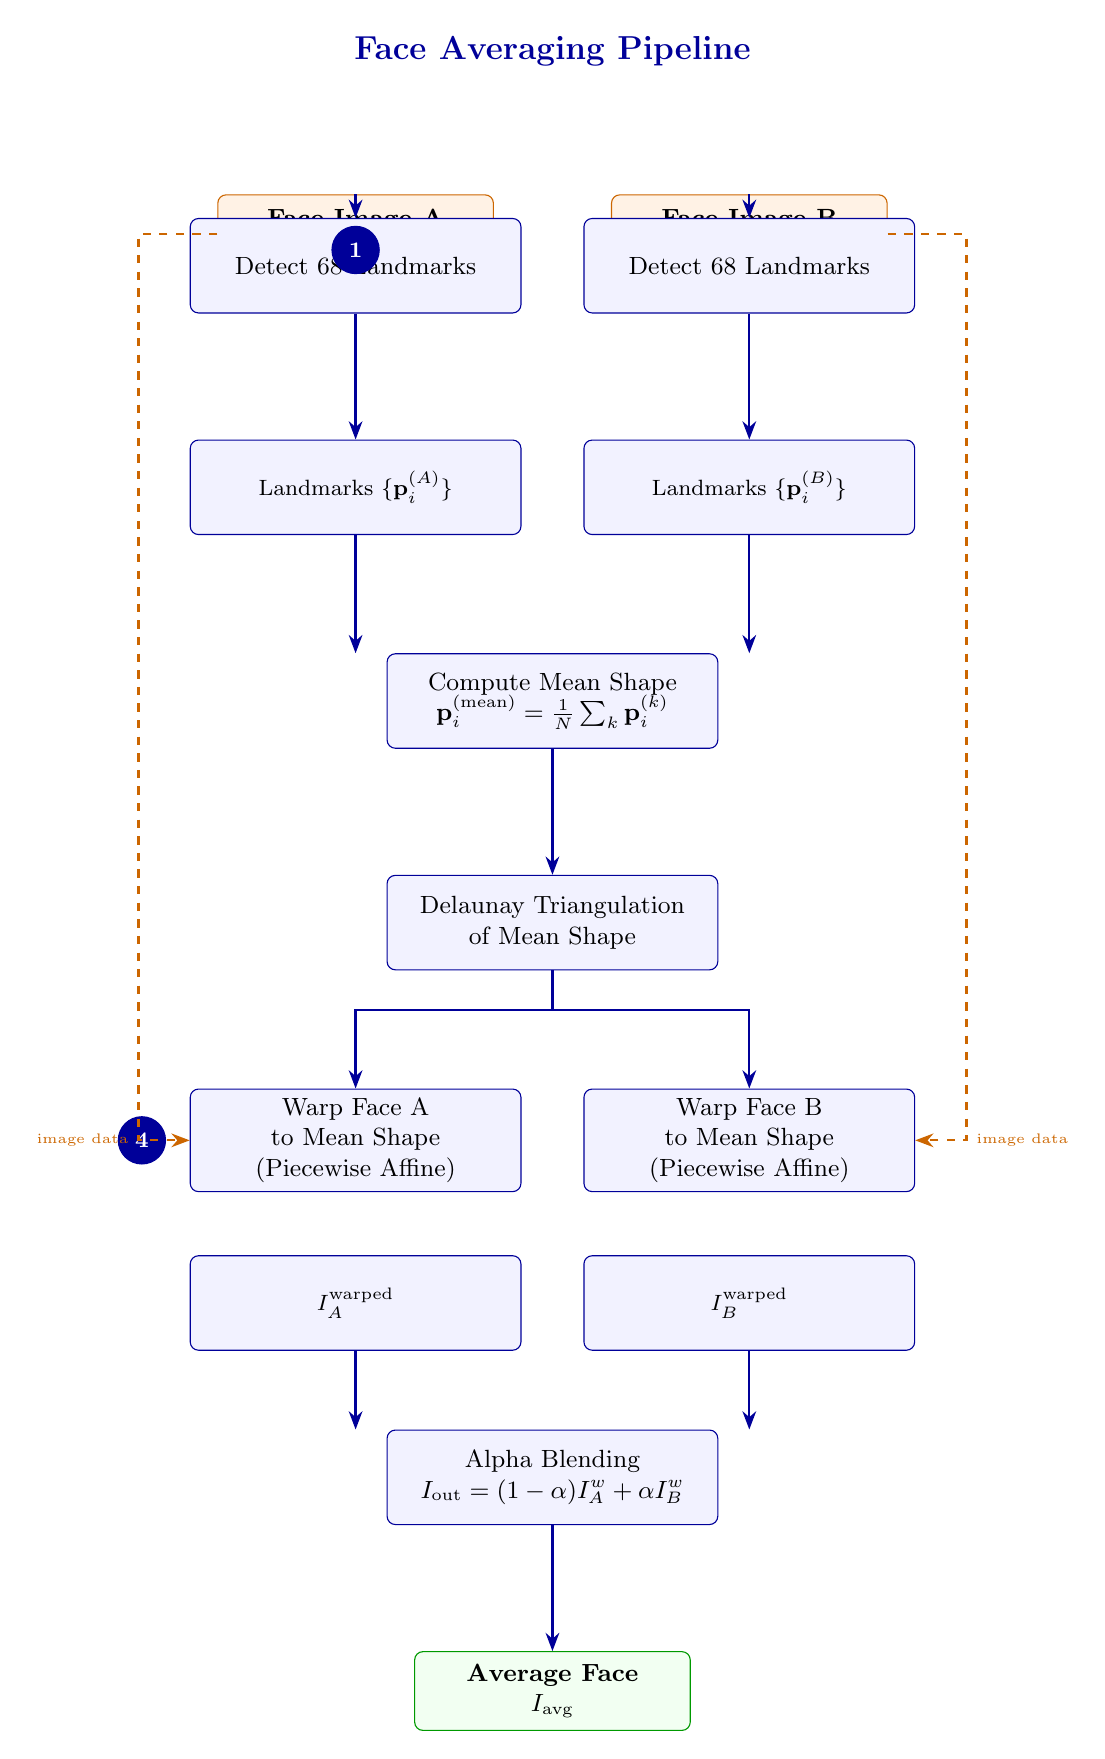
\begin{tikzpicture}[
        >=Stealth,
        node distance=1.6cm,
        box/.style={
            rectangle,
            rounded corners=3pt,
            draw=blue!60!black,
            fill=blue!5,
            minimum width=4.2cm,
            minimum height=1.2cm,
            align=center,
            font=\small
        },
        inputbox/.style={
            rectangle,
            rounded corners=3pt,
            draw=orange!80!black,
            fill=orange!10,
            minimum width=3.5cm,
            minimum height=1.0cm,
            align=center,
            font=\small
        },
        outputbox/.style={
            rectangle,
            rounded corners=3pt,
            draw=green!60!black,
            fill=green!5,
            minimum width=3.5cm,
            minimum height=1.0cm,
            align=center,
            font=\small
        },
        stepnum/.style={
            circle,
            draw=blue!60!black,
            fill=blue!60!black,
            text=white,
            minimum size=0.6cm,
            font=\footnotesize\bfseries,
            inner sep=0pt
        },
        arrow/.style={
            ->,
            thick,
            blue!60!black
        }
    ]
    % Title
    \node[font=\large\bfseries, text=blue!60!black] (title)
        {Face Averaging Pipeline};

    % Input faces (parallel branches)
    \node[inputbox, below=1.5cm of title, xshift=-2.5cm] (faceA)
        {\textbf{Face Image A}\\$I_A$};
    \node[inputbox, below=1.5cm of title, xshift=2.5cm] (faceB)
        {\textbf{Face Image B}\\$I_B$};

    % Step 1: Landmark Detection
    \node[box, below=1.8cm of title, xshift=-2.5cm] (step1a)
        {Detect 68 Landmarks};
    \node[box, below=1.8cm of title, xshift=2.5cm] (step1b)
        {Detect 68 Landmarks};
    \node[stepnum, at={($(faceA)!0.5!(step1a)$)}] (s1label) {1};

    % Landmark outputs
    \node[box, below=of step1a, font=\footnotesize] (landA)
        {Landmarks $\{\mathbf{p}^{(A)}_i\}$};
    \node[box, below=of step1b, font=\footnotesize] (landB)
        {Landmarks $\{\mathbf{p}^{(B)}_i\}$};

    % Step 2: Mean Shape
    \node[box, below=1.5cm of landA, xshift=2.5cm] (step2)
        {Compute Mean Shape\\$\mathbf{p}^{(\text{mean})}_i = \frac{1}{N}\sum_k
        \mathbf{p}^{(k)}_i$};

    % Step 3: Triangulation
    \node[box, below=of step2] (step3)
        {Delaunay Triangulation\\of Mean Shape};

    % Step 4: Warping (two parallel paths)
    \node[box, below=1.5cm of step3, xshift=-2.5cm] (step4a)
        {Warp Face A\\to Mean Shape\\(Piecewise Affine)};
    \node[box, below=1.5cm of step3, xshift=2.5cm] (step4b)
        {Warp Face B\\to Mean Shape\\(Piecewise Affine)};
    \node[stepnum, left=3mm of step4a] () {4};

    \node[box, below=0.8cm of step4a, font=\footnotesize] (warpA)
        {$I_A^{\text{warped}}$};
    \node[box, below=0.8cm of step4b, font=\footnotesize] (warpB)
        {$I_B^{\text{warped}}$};

    % Step 5: Blending
    \node[box, below=1.0cm of warpA, xshift=2.5cm] (step5)
        {Alpha Blending\\$I_{\text{out}} = (1-\alpha) I_A^w + \alpha I_B^w$};

    % Output
    \node[outputbox, below=of step5] (output)
        {\textbf{Average Face}\\$I_{\text{avg}}$};

    % Arrows: Face -> Landmark Detection
    \draw[arrow] (faceA) -- (step1a);
    \draw[arrow] (faceB) -- (step1b);

    % Arrows: Landmark Detection -> Landmark outputs
    \draw[arrow] (step1a) -- (landA);
    \draw[arrow] (step1b) -- (landB);

    % Arrows: Landmarks -> Mean Shape
    \draw[arrow] (landA) -- (landA |- step2.north);
    \draw[arrow] (landB) -- (landB |- step2.north);

    % Arrow: Mean Shape -> Triangulation
    \draw[arrow] (step2) -- (step3);

    % Arrows: Triangulation -> Warping
    \draw[arrow] (step3.south) -- +(0, -0.5cm) -| (step4a.north);
    \draw[arrow] (step3.south) -- +(0, -0.5cm) -| (step4b.north);

    % Arrow: Face A -> Warp A (implicit: use same triangulation)
    \draw[arrow, dashed, orange!80!black] (faceA.west) -- ++(-1.0cm, 0) |- (step4a.west)
        node[midway, left, font=\tiny, text=orange!80!black] {image data};
    \draw[arrow, dashed, orange!80!black] (faceB.east) -- ++(1.0cm, 0) |- (step4b.east)
        node[midway, right, font=\tiny, text=orange!80!black] {image data};

    % Arrows: Warped -> Blending
    \draw[arrow] (warpA) -- (warpA |- step5.north);
    \draw[arrow] (warpB) -- (warpB |- step5.north);

    % Arrow: Blending -> Output
    \draw[arrow] (step5) -- (output);

    \end{tikzpicture}
    \caption{Complete face averaging pipeline. Two input face images (orange, top) are processed
    in parallel through landmark detection. The extracted landmark sets are combined to compute a
    mean shape (Step~2), which is then triangulated using Delaunay triangulation (Step~3).
    The triangulation guides piecewise affine warping of each face into the mean geometry
    (Step~4). Finally, the warped images are blended via alpha compositing (Step~5) to produce
    the output average face (green, bottom). Dashed orange arrows indicate that the original
    image pixel data flows directly into the warping stage, guided by the geometric structure
    computed in Steps 2 and 3.}
    \label{fig:pipeline}
\end{figure}

\subsection{Why This Approach Produces Natural Results}

To close this introduction, it is worth understanding at an intuitive level why the feature-based
approach succeeds where the naive approach fails.

The core reason is \emph{structural alignment}. When a human observer looks at a face, the brain
does not process it pixel by pixel. Instead, it identifies a structure: there are two eyes, a nose,
a mouth, arranged in a particular configuration. The recognition and interpretation of the face
depends on getting this structure right.

The naive pixel-averaging approach operates at the level of the retina (the pixel grid), ignoring
structure entirely. It assumes that pixel $(x, y)$ in one face corresponds to pixel $(x, y)$ in
the other face, which is simply not true for any features beyond the alignment anchors.

The feature-based approach, by contrast, operates at the level of the structure. By identifying
corresponding landmarks and warping to a common geometry, we ensure that the left eye of Face A
and the left eye of Face B are mapped to the same location in the output before their pixel
values are averaged. The structure is aligned first, so the pixel averaging makes sense.

The result is a face that looks like a real person because the internal structure is internally
consistent. All features are in their proper relative positions, just as they would be in a
photograph. The eyes are sharp because both input eye images have been warped to the same
geometry before averaging, rather than being averaged at slightly offset positions. The same is
true for the nose, mouth, and all other features.

This structural perspective also explains why 68 landmarks (or similar) are sufficient to produce
convincing results even though a typical face image contains millions of pixels. The landmarks
capture the essential structural degrees of freedom of the face --- the positions of eyes, nose,
mouth, jaw, and eyebrows --- and the piecewise affine warping fills in the continuous deformation
between these control points. The pixel values carry the texture and color information, but the
structure is entirely determined by the landmarks.

In the following sections, we will examine each of these five pipeline steps in detail, working
through the mathematics, the implementation, and the design choices that go into building a
complete face morphing system.


\endinput

\section{Facial Landmark Detection}

Before we can morph one face into another, we need to know \emph{where} the key facial features are located in each image. This is the job of \textbf{facial landmark detection}.

\subsection{What Are Facial Landmarks?}

Facial landmarks are \textbf{semantically meaningful points} on a face. Each landmark marks an anatomically identifiable location, such as:

\begin{itemize}
    \item The corners of the eyes (inner and outer canthus)
    \item The tip and nostrils of the nose
    \item The corners and midpoints of the lips
    \item The outer boundary of the jawline
    \item The arcs of the eyebrows
\end{itemize}

Why do we need them? Because face morphing is fundamentally about establishing \textbf{correspondence}: for every pixel on face~A, we need to know which pixel on face~B plays the same anatomical role. Landmarks give us a sparse set of anchor points that define this correspondence.

\begin{definition}[Corresponding Points]
    Two landmarks $p_i^{(A)}$ and $p_i^{(B)}$ on two different faces are called \textbf{corresponding points} if they refer to the \textbf{same anatomical location}. For example, the left eye corner on face~A corresponds to the left eye corner on face~B, both carrying index~$i = 36$ in the standard 68-point model.
\end{definition}

When we average two faces, we compute intermediate positions for each corresponding landmark and warp the images so that these intermediate positions are aligned. The quality of the morph depends critically on having accurate, well-matched landmarks.

\subsection{The 68-Point Landmark Model}

The most widely used landmark model comes from the \textbf{iBUG 300-W dataset}~\footnote{The iBUG 300-W dataset is a widely used benchmark for facial landmark detection.}. It defines exactly 68 points per face, organized into nine anatomical regions. This model was trained on thousands of annotated face images and has become a de facto standard in academic and practical work.

\subsubsection*{Point Groups}

Table~\ref{tab:landmark-regions} lists every region with its index range, number of points, and a brief description.

\begin{table}[htbp]
    \centering
    \caption{Mapping of index ranges to facial regions in the 68-point model}
    \label{tab:landmark-regions}
    \begin{tabular}{@{} l c c p{6cm} @{}}
        \toprule
        \textbf{Region} & \textbf{Indices} & \textbf{\# Points} & \textbf{Description} \\
        \midrule
        Jawline & 0--17 & 18 & Points along the chin contour, from left ear to right ear \\
        Left eyebrow & 17--21 & 5 & Arc from inner to outer left brow \\
        Right eyebrow & 22--26 & 5 & Arc from inner to outer right brow \\
        Nose bridge & 27--30 & 4 & Vertical line down the centre of the nose \\
        Nose base & 31--35 & 5 & Nostril edges and nose tip, left to right \\
        Left eye & 36--41 & 6 & Upper and lower eyelid of the left eye \\
        Right eye & 42--47 & 6 & Upper and lower eyelid of the right eye \\
        Outer mouth & 48--59 & 12 & Outer lip contour (upper + lower lip) \\
        Inner mouth & 60--67 & 8 & Inner lip contour (vermilion border) \\
        \bottomrule
    \end{tabular}
\end{table}

\paragraph*{Detailed descriptions.}

\textbf{Jawline (0--17).} These 18 points trace the lower boundary of the face. Point~0 sits near the left ear, point~17 near the right ear, and the midpoint (indices 8--9) falls at the chin. This contour is critical for aligning face shapes during morphing.

\textbf{Eyebrows (17--26).} Each eyebrow is modelled as a simple five-point arc. The left eyebrow runs from the inner corner (index~17, near the nose bridge) to the outer edge (index~21). The right eyebrow mirrors this from inner (index~22) to outer (index~26).

\textbf{Nose (27--35).} The nose is divided into the bridge (27--30) and the base (31--35). Point~27 starts at the top of the nose bridge between the eyebrows; points~28--30 descend along the bridge; points~31--35 spread across the nostrils and nose tip, with point~33 at the nose centre.

\textbf{Eyes (36--47).} Each eye is represented by six points forming a hexagon:
\begin{itemize}
    \item Point~36: left eye outer corner, Point~38: upper eyelid midpoint, Point~39: left eye inner corner
    \item Point~40: lower eyelid midpoint-left, Point~41: lower eyelid midpoint-right
    \item Points~42--47 mirror this for the right eye
\end{itemize}

\textbf{Mouth (48--67).} The outer mouth (48--59) traces the visible lip border with 12 points (6 on the upper lip, 6 on the lower lip). The inner mouth (60--67) traces the vermilion border \emph{inside} the lips, which helps capture mouth opening and expression changes.

\subsubsection*{Schematic Diagram}

Figure~\ref{fig:landmark-68} shows a schematic face outline with all 68 landmark points labelled.

\begin{figure}[htbp]
    \centering
    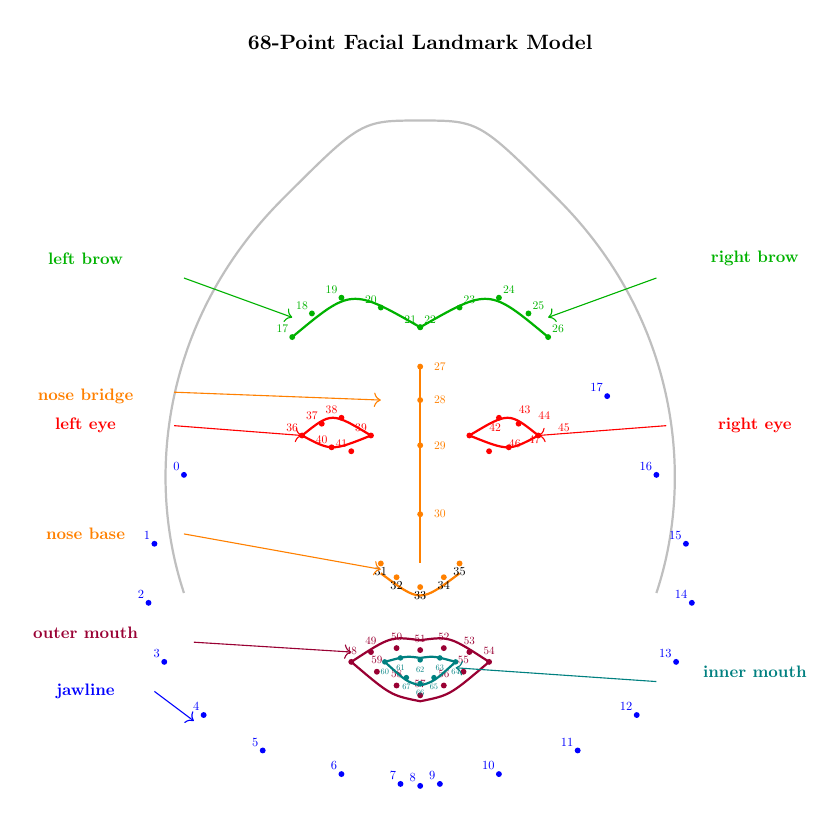
\begin{tikzpicture}[scale=2.5]
        % Face outline (jaw + forehead suggestion)
        \draw[color=gray!50, thick]
            (-1.2, -0.2) .. controls (-1.4, 0.4) and (-1.3, 1.2) .. (-0.7, 1.8)
            .. controls (-0.3, 2.2) .. (0, 2.2)
            .. controls (0.3, 2.2) .. (0.7, 1.8)
            .. controls (1.3, 1.2) and (1.4, 0.4) .. (1.2, -0.2);

        % Jawline points (0-17) — along the lower contour
        \foreach \i/\x/\y in {
            0/-1.2/0.4, 1/-1.35/0.05, 2/-1.38/-0.25, 3/-1.3/-0.55,
            4/-1.1/-0.82, 5/-0.8/-1.0, 6/-0.4/-1.12, 7/-0.1/-1.17,
            8/0/-1.18, 9/0.1/-1.17, 10/0.4/-1.12, 11/0.8/-1.0,
            12/1.1/-0.82, 13/1.3/-0.55, 14/1.38/-0.25, 15/1.35/0.05,
            16/1.2/0.4, 17/0.95/0.8
        }{
            \fill[blue] (\x,\y) circle (0.015);
            \node[scale=0.45, blue, anchor=south east] at (\x,\y) {\i};
        }

        % Left eyebrow (17-21)
        \draw[color=green!70!black, thick] (-0.65, 1.1) .. controls (-0.35, 1.35) .. (0.0, 1.15);
        \foreach \i/\x/\y in {
            17/-0.65/1.1, 18/-0.55/1.22, 19/-0.4/1.3, 20/-0.2/1.25, 21/0.0/1.15
        }{
            \fill[green!70!black] (\x,\y) circle (0.015);
            \node[scale=0.42, green!70!black, anchor=south east] at (\x,\y) {\i};
        }

        % Right eyebrow (22-26)
        \draw[color=green!70!black, thick] (0.0, 1.15) .. controls (0.35, 1.35) .. (0.65, 1.1);
        \foreach \i/\x/\y in {
            22/0.0/1.15, 23/0.2/1.25, 24/0.4/1.3, 25/0.55/1.22, 26/0.65/1.1
        }{
            \fill[green!70!black] (\x,\y) circle (0.015);
            \node[scale=0.42, green!70!black, anchor=south west] at (\x,\y) {\i};
        }

        % Nose bridge (27-30)
        \draw[color=orange, thick] (0, 0.95) -- (0, 0.55) -- (0, 0.2) -- (0, -0.05);
        \foreach \i/\x/\y in {
            27/0/0.95, 28/0/0.78, 29/0/0.55, 30/0/0.2
        }{
            \fill[orange] (\x,\y) circle (0.015);
            \node[scale=0.42, orange, anchor=west] at (\x+0.05,\y) {\i};
        }

        % Nose base (31-35)
        \draw[color=orange, thick] (-0.2,-0.1) .. controls (0,-0.25) .. (0.2,-0.1);
        \foreach \i/\x/\y in {
            31/-0.2/-0.05, 32/-0.12/-0.12, 33/0/-0.17, 34/0.12/-0.12, 35/0.2/-0.05
        }{
            \fill[orange] (\x,\y) circle (0.015);
            \node[scale=0.44, anchor=north] at (\x,\y) {\i};
        }

        % Left eye (36-41)
        \draw[color=red, thick]
            (-0.6, 0.6) .. controls (-0.45, 0.72) .. (-0.25, 0.6)
            .. controls (-0.45, 0.52) .. (-0.6, 0.6);
        \foreach \i/\x/\y in {
            36/-0.6/0.6, 37/-0.5/0.66, 38/-0.4/0.69, 39/-0.25/0.6,
            40/-0.45/0.54, 41/-0.35/0.52
        }{
            \fill[red] (\x,\y) circle (0.015);
            \node[scale=0.42, red, anchor=south east] at (\x,\y) {\i};
        }

        % Right eye (42-47)
        \draw[color=red, thick]
            (0.25, 0.6) .. controls (0.45, 0.72) .. (0.6, 0.6)
            .. controls (0.45, 0.52) .. (0.25, 0.6);
        \foreach \i/\x/\y in {
            42/0.25/0.6, 43/0.4/0.69, 44/0.5/0.66, 45/0.6/0.6,
            46/0.35/0.52, 47/0.45/0.54
        }{
            \fill[red] (\x,\y) circle (0.015);
            \node[scale=0.42, red, anchor=south west] at (\x+0.08,\y) {\i};
        }

        % Outer mouth (48-59)
        \draw[color=purple!80!black, thick]
            (-0.35, -0.55) .. controls (-0.15, -0.42) .. (0, -0.44)
            .. controls (0.15, -0.42) .. (0.35, -0.55)
            .. controls (0.15, -0.72) .. (0, -0.75)
            .. controls (-0.15, -0.72) .. (-0.35, -0.55);
        \foreach \i/\x/\y in {
            48/-0.35/-0.55, 49/-0.25/-0.50, 50/-0.12/-0.48, 51/0/-0.49,
            52/0.12/-0.48, 53/0.25/-0.50, 54/0.35/-0.55,
            55/0.22/-0.60, 56/0.12/-0.67, 57/0/-0.72,
            58/-0.12/-0.67, 59/-0.22/-0.60
        }{
            \fill[purple!80!black] (\x,\y) circle (0.015);
            \node[scale=0.4, purple!80!black, anchor=south] at (\x,\y+0.02) {\i};
        }

        % Inner mouth (60-67)
        \draw[color=teal, thick]
            (-0.18, -0.55) .. controls (-0.07, -0.52) .. (0, -0.53)
            .. controls (0.07, -0.52) .. (0.18, -0.55)
            .. controls (0.07, -0.65) .. (0, -0.67)
            .. controls (-0.07, -0.65) .. (-0.18, -0.55);
        \foreach \i/\x/\y in {
            60/-0.18/-0.55, 61/-0.10/-0.53, 62/0/-0.54, 63/0.10/-0.53,
            64/0.18/-0.55, 65/0.07/-0.63, 66/0/-0.66, 67/-0.07/-0.63
        }{
            \fill[teal] (\x,\y) circle (0.014);
            \node[scale=0.3, teal, anchor=north] at (\x,\y-0.02) {\i};
        }

        % Region labels with arrows
        \node[blue, scale=0.6, font=\bfseries] at (-1.7, -0.7) {jawline};
        \draw[blue, ->, thin] (-1.35, -0.7) -- (-1.15, -0.85);

        \node[green!70!black, scale=0.6, font=\bfseries] at (-1.7, 1.5) {left brow};
        \draw[green!70!black, ->, thin] (-1.2, 1.4) -- (-0.65, 1.2);

        \node[green!70!black, scale=0.6, font=\bfseries] at (1.7, 1.5) {right brow};
        \draw[green!70!black, ->, thin] (1.2, 1.4) -- (0.65, 1.2);

        \node[orange, scale=0.6, font=\bfseries] at (-1.7, 0.8) {nose bridge};
        \draw[orange, ->, thin] (-1.25, 0.82) -- (-0.2, 0.78);

        \node[orange, scale=0.6, font=\bfseries] at (-1.7, 0.1) {nose base};
        \draw[orange, ->, thin] (-1.2, 0.1) -- (-0.2, -0.08);

        \node[red, scale=0.6, font=\bfseries] at (-1.7, 0.65) {left eye};
        \draw[red, ->, thin] (-1.25, 0.65) -- (-0.6, 0.6);

        \node[red, scale=0.6, font=\bfseries] at (1.7, 0.65) {right eye};
        \draw[red, ->, thin] (1.25, 0.65) -- (0.6, 0.6);

        \node[purple!80!black, scale=0.6, font=\bfseries] at (-1.7, -0.4) {outer mouth};
        \draw[purple!80!black, ->, thin] (-1.15, -0.45) -- (-0.35, -0.50);

        \node[teal, scale=0.6, font=\bfseries] at (1.7, -0.6) {inner mouth};
        \draw[teal, ->, thin] (1.2, -0.65) -- (0.18, -0.58);

        % Title
        \node[font=\bfseries, scale=0.75] at (0, 2.6) {68-Point Facial Landmark Model};
    \end{tikzpicture}
    \caption{Schematic diagram of the 68-point facial landmark model. Each colour corresponds to a different facial region. Points are numbered according to the iBUG 300-W convention.}
    \label{fig:landmark-68}
\end{figure}

\subsection{How Landmark Detectors Work}

Landmark detection algorithms take an image (or a cropped face region) as input and output a set of 2D coordinates $\{(x_i, y_i)\}_{i=0}^{67}$ for the 68-point model. Three approaches are particularly noteworthy.

\subsubsection*{HOG + SVM + Regressed Trees (dlib Classic)}

This pipeline, popularized by the widely used \texttt{dlib} library~\footnote{See the dlib library documentation for details on the HOG+SVM face detector.}, works in two stages:

\begin{enumerate}
    \item \textbf{Face detection with HOG + linear SVM.} A \textbf{Histogram of Oriented Gradients} feature descriptor is computed on sliding windows across the image. Each window's HOG feature vector is classified by a \textbf{Support Vector Machine} trained to distinguish face regions from background. The result is a bounding box around the detected face.
    \item \textbf{Landmark localization with cascaded regression.} Given the bounding box, a cascade of \textbf{regression trees} iteratively refines the landmark positions. Starting from an initial estimate (often the mean shape from the training data), each tree in the cascade predicts a correction $\Delta$ to the current landmark positions:
    \begin{equation}
        \mathbf{s}_{t+1} = \mathbf{s}_t + \Delta_t(\mathbf{I}, \mathbf{s}_t),
    \end{equation}
    where $\mathbf{s}_t$ is the shape at iteration $t$, $\mathbf{I}$ is the image, and $\Delta_t$ is the $t$-th regressor's prediction. After typically 5--10 iterations, the landmarks converge to stable positions.
\end{enumerate}

\textbf{Pros:} Very fast (runs in real time on a CPU), small model size. \\
\textbf{Cons:} Less accurate than deep learning methods, especially for non-frontal faces or unusual expressions.

\subsubsection*{Deep Neural Network (dlib CNN)}

The same \texttt{dlib} library also provides a CNN-based landmark detector~\footnote{One Millisecond Face Alignment with an Ensemble of Regression Trees, Kazemi \& Sullivan, CVPR 2014.}. This model replaces the hand-crafted HOG features and decision-tree cascade with a single \textbf{end-to-end convolutional neural network} that takes a normalized face patch as input and directly outputs the 68 landmark coordinates (136 real values).

Because the network learns features from data rather than relying on histogram statistics, it is significantly more robust to variations in lighting, pose, and expression.

\textbf{Pros:} Higher accuracy, better handling of partial occlusions and extreme poses. \\
\textbf{Cons:} Slower than the HOG-based approach (though still CPU-feasible), larger model footprint.

\subsubsection*{MediaPipe Face Mesh (Google)}

Google's MediaPipe framework~\footnote{MediaPipe is Google's open-source framework for multimodal ML models, including real-time face mesh detection.} takes a different approach: instead of 68 points, it predicts \textbf{477 3D facial landmarks}, providing much denser coverage across the entire face surface. It uses a multi-stage pipeline:

\begin{enumerate}
    \item \textbf{BlazeFace detector:} A lightweight neural network quickly locates the face and produces a rough bounding box (with sub-millisecond latency).
    \item \textbf{Face Mesh model:} A deeper CNN takes the cropped face region and predicts the full 477-point mesh, including 3D coordinates $(x, y, z)$ where $z$ represents depth relative to the image plane.
\end{enumerate}

The 477 points cover the entire facial surface: contours, eyes, eyebrows, nose, lips, teeth, and even sub-regions of the iris. This density is useful for high-fidelity morphing and augmented reality, though it introduces additional computational complexity.

\textbf{Pros:} Extremely dense coverage, 3D depth information, real-time on mobile devices, robust across diverse lighting and pose conditions. \\
\textbf{Cons:} Overkill for basic morphing (most morphing workflows only need $\sim$68 points), output must be subsampled or mapped to the 68-point convention for compatibility.

\subsection{Coordinate System}

All landmark coordinates are expressed in the standard \textbf{image coordinate system}. Unlike the Cartesian coordinate system taught in mathematics class, image coordinates have the following convention:

\begin{itemize}
    \item The \textbf{origin} $(0, 0)$ is at the \textbf{top-left corner} of the image.
    \item The $x$-axis increases \textbf{rightward}.
    \item The $y$-axis increases \textbf{downward}.
\end{itemize}

Landmark coordinates are stored as \textbf{floating-point values in pixel units}. This means that a landmark at $(x, y) = (150.5, 200.3)$ refers to a sub-pixel location 150.5~pixels from the left edge and 200.3~pixels from the top edge. Sub-pixel precision is important because warping operations work with fractional coordinates.

Figure~\ref{fig:coord-system} illustrates this coordinate system.

\begin{figure}[htbp]
    \centering
    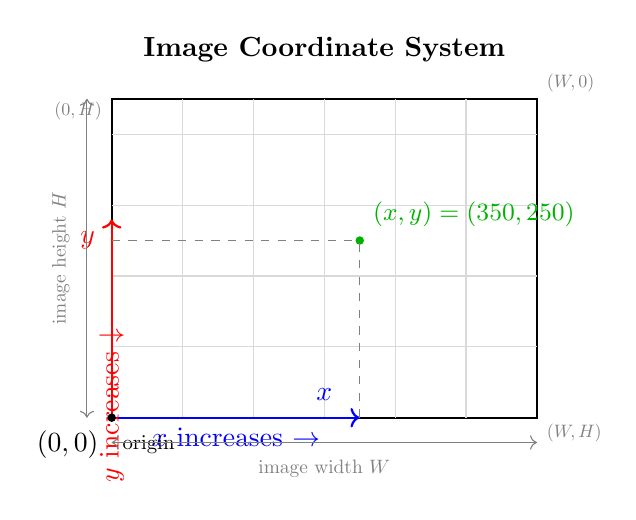
\begin{tikzpicture}[scale=0.9]
        % Image rectangle
        \draw[thick] (0,0) rectangle (6,4.5);

        % Grid lines (subtle)
        \foreach \x in {1,...,5} {
            \draw[gray!30] (\x,0) -- (\x,4.5);
        }
        \foreach \y in {1,...,4} {
            \draw[gray!30] (0,\y) -- (6,\y);
        }

        % Axes
        \draw[->, thick, blue] (0,0) -- (3.5,0) node[midway, below, sloped] {$x$ increases \(\rightarrow\)};
        \draw[->, thick, red] (0,0) -- (0,2.8) node[midway, left, sloped] {$y$ increases \(\downarrow\)};

        % Origin
        \fill[black] (0,0) circle (0.06);
        \node[anchor=north east, font=\bfseries] at (-0.05, -0.05) {$(0,0)$};
        \node[anchor=north west, scale=0.75] at (0.05, -0.15) {origin};

        % Axis labels
        \node[anchor=south, blue, font=\bfseries] at (3,0.1) {$x$};
        \node[anchor=east, red, font=\bfseries] at (-0.1,2.5) {$y$};

        % Example landmark point
        \fill[green!70!black] (3.5,2.5) circle (0.06);
        \node[anchor=south west, green!70!black, font=\small] at (3.55, 2.55) {\small$(x, y) = (350, 250)$};
        \draw[dashed, gray] (3.5,0) -- (3.5,2.5);
        \draw[dashed, gray] (0,2.5) -- (3.5,2.5);

        % Pixel dimensions annotation
        \node[anchor=north, gray, scale=0.7] at (3, -0.5) {image width $W$};
        \draw[gray, <->] (0, -0.35) -- (6, -0.35);
        \node[anchor=east, gray, scale=0.7] at (-0.5, 2.25) {\rotatebox{90}{image height $H$}};
        \draw[gray, <->] (-0.35, 0) -- (-0.35, 4.5);

        % Top-right corner
        \node[anchor=south west, gray, scale=0.65] at (6.05, 4.5) {$(W, 0)$};
        \node[anchor=north west, gray, scale=0.65] at (6.05, 0) {$(W, H)$};
        \node[anchor=north east, gray, scale=0.65] at (-0.05, 4.55) {$(0, H)$};

        % Title
        \node[font=\bfseries] at (3, 5.2) {Image Coordinate System};
    \end{tikzpicture}
    \caption{The image coordinate system used for landmarks. The origin is at the top-left corner, $x$ increases rightward, and $y$ increases downward. An example landmark at $(350, 250)$ is shown in green.}
    \label{fig:coord-system}
\end{figure}

\begin{remark}
    When working with multiple detector libraries, be aware of coordinate conventions. Some libraries return landmarks in \emph{normalized} coordinates $[0, 1]$ relative to the face bounding box, rather than absolute pixel coordinates. Always check the API documentation and convert coordinates to your preferred frame before warping.
\end{remark}

\subsection{Preprocessing for Better Detection}

Landmark detectors are sensitive to the quality of the input face image. Although modern detectors are fairly robust, following a few simple preprocessing guidelines will significantly improve detection accuracy \emph{and} downstream morphing quality.

\paragraph*{Why good face detection and cropping matters.}

All landmark models are trained on face images that share certain properties:
\begin{itemize}
    \item \textbf{The face is roughly front-facing.} Extreme side profiles (more than $\sim45^\circ$ rotation) cause many landmarks to be occluded and therefore poorly localized.
    \item \textbf{The face is large enough in the frame.} As a rule of thumb, the cropped face should be at least $200 \times 200$ pixels. Below this, pixel-level detail around the eyes, lips, and nose is insufficient for precise localization.
    \item \textbf{The face is roughly centred and upright.} Large in-plane rotations (tilting your head sideways) confuse detectors because the statistical priors assume an upright face.
\end{itemize}

A typical preprocessing pipeline for morphing therefore looks like this:
\begin{enumerate}
    \item \textbf{Detect} the face bounding box (using any face detector).
    \item \textbf{Crop} a square region around the face with some margin (e.g., 20\% padding on each side).
    \item \textbf{Align} by rotating the image so that the eyes are horizontally level. This can be done by computing the angle $\theta = \arctan\!\big((y_R - y_L)/(x_R - x_L)\big)$ between the two eye centres and applying a rotation.
    \item \textbf{Resize} to a standard resolution (e.g., $512 \times 512$ pixels) so that landmark coordinates are comparable across images.
    \item \textbf{Run the landmark detector} on the preprocessed face.
\end{enumerate}

The result is a set of landmarks that are accurate, consistent, and ready for computing the correspondence needed to morph two faces together---the subject of the next section.

\section{Geometric Foundations}

Feature-based face morphing requires us to deform one facial geometry so that landmarks align with those of another face.  The workhorse for this deformation is the \emph{piecewise affine warp}: we triangulate the landmark sets, then apply an affine transformation to each corresponding triangle pair.  In this section we build the full mathematical machinery --- affine transformations, barycentric coordinates, and inverse mapping --- that makes the warp both exact and hole-free.

%-----------------------------------------------------------------------
\subsection{Affine Transformations --- Theory}
%-----------------------------------------------------------------------

An \textbf{affine transformation} in 2D is a mapping
\[
    f : \mathbb{R}^2 \to \mathbb{R}^2,
    \qquad f(\mathbf{x}) = \mathbf{A}\,\mathbf{x} + \mathbf{t},
\]
where $\mathbf{A} \in \mathbb{R}^{2 \times 2}$ is a linear transformation matrix and $\mathbf{t} \in \mathbb{R}^2$ is a translation vector.  Written component-wise for a point $(x, y)$ mapped to $(x', y')$:
\[
\begin{bmatrix} x' \\ y' \end{bmatrix}
=
\begin{bmatrix}
    a_{11} & a_{12} \\
    a_{21} & a_{22}
\end{bmatrix}
\begin{bmatrix} x \\ y \end{bmatrix}
+
\begin{bmatrix} t_x \\ t_y \end{bmatrix}.
\]

\paragraph{Key properties.}
An affine transformation preserves:
\begin{itemize}
    \item \textbf{Collinearity:} three points on a line remain on a line.
    \item \textbf{Parallelism:} parallel lines remain parallel.
    \item \textbf{Ratios of distances along a line:} if $C$ divides segment $AB$ in ratio $r\!:\!(1-r)$, the image $C'$ divides $A'B'$ in the same ratio.
\end{itemize}
It does \emph{not} preserve angles or absolute lengths unless $\mathbf{A}$ happens to be a pure rotation.

\paragraph{Matrix form with homogeneous coordinates.}
It is convenient to embed a 2D point as a 3-vector $(x,\,y,\,1)^\top$ and write the transform as a single $3\times3$ matrix multiplication:
\[
\begin{bmatrix} x' \\ y' \\ 1 \end{bmatrix}
=
\begin{bmatrix}
    a_{11} & a_{12} & t_x \\
    a_{21} & a_{22} & t_y \\
    0      & 0      & 1
\end{bmatrix}
\begin{bmatrix} x \\ y \\ 1 \end{bmatrix}.
\]
The bottom row $(0,\,0,\,1)$ ensures the homogeneous coordinate remains 1, so the result always corresponds to a genuine 2D point.  We discuss homogeneous coordinates in more depth in Section~\ref{sec:homogeneous}.

\paragraph{Geometric decomposition of the linear submatrix.}
The $2\times2$ matrix $\mathbf{A}$ can be decomposed into elementary geometric operations.  One useful decomposition is
\[
    \mathbf{A} = \mathbf{R}(\theta)\; \mathbf{S}\; \mathbf{H},
\]
where:
\begin{align*}
    \mathbf{R}(\theta) &=
    \begin{bmatrix}
        \cos\theta & -\sin\theta \\
        \sin\theta &  \cos\theta
    \end{bmatrix}
    && \text{(rotation by $\theta$)}, \\[6pt]
    \mathbf{S} &=
    \begin{bmatrix}
        s_x & 0 \\
        0   & s_y
    \end{bmatrix}
    && \text{(anisotropic scaling)}, \\[6pt]
    \mathbf{H} &=
    \begin{bmatrix}
        1 & h \\
        0 & 1
    \end{bmatrix}
    && \text{(horizontal shear)}.
\end{align*}
Other orderings are possible; the important point is that any invertible $2\times2$ matrix can be factored this way, so an affine transform can always be interpreted as a sequence of rotation, anisotropic scaling, shear, and translation.

\paragraph{Degrees of freedom.}
An affine transformation in 2D has exactly \textbf{six} free parameters: the four entries of $\mathbf{A}$ ($a_{11}, a_{12}, a_{21}, a_{22}$) and the two translation components ($t_x, t_y$).  This means six independent constraints uniquely determine the transform --- and, as we will see next, three point correspondences provide exactly six scalar equations.

%-----------------------------------------------------------------------
\subsection{Computing Affine Transforms from Three Point Correspondences}
%-----------------------------------------------------------------------

\begin{theorem}
An affine transformation in 2D is uniquely determined by three non-collinear point correspondences.
\end{theorem}

\begin{proof}
Let the source triangle have vertices $\mathbf{P}_1, \mathbf{P}_2, \mathbf{P}_3 \in \mathbb{R}^2$ and the corresponding destination vertices be $\mathbf{Q}_1, \mathbf{Q}_2, \mathbf{Q}_3$.  We seek $\mathbf{A}$ and $\mathbf{t}$ such that
\[
    \mathbf{Q}_i = \mathbf{A}\,\mathbf{P}_i + \mathbf{t}, \qquad i = 1,2,3.
\]

Introduce homogeneous coordinates by augmenting each point with a trailing 1, and assemble the three points column-wise into $3\times3$ matrices:
\[
    \mathbf{P}_{\mathrm{h}} =
    \begin{bmatrix}
        x_1 & x_2 & x_3 \\
        y_1 & y_2 & y_3 \\
        1   & 1   & 1
    \end{bmatrix},
    \qquad
    \mathbf{Q}_{\mathrm{h}} =
    \begin{bmatrix}
        x'_1 & x'_2 & x'_3 \\
        y'_1 & y'_2 & y'_3 \\
        1    & 1    & 1
    \end{bmatrix}.
\]
The affine transform in homogeneous form is
\[
    \mathbf{T} =
    \begin{bmatrix}
        a_{11} & a_{12} & t_x \\
        a_{21} & a_{22} & t_y \\
        0      & 0      & 1
    \end{bmatrix},
\]
and the three correspondences are captured compactly as
\[
    \mathbf{Q}_{\mathrm{h}} = \mathbf{T}\,\mathbf{P}_{\mathrm{h}}.
\]
Because the three source points are non-collinear, $\mathbf{P}_{\mathrm{h}}$ has full rank (its determinant equals twice the signed area of the triangle, which is nonzero).  Therefore $\mathbf{P}_{\mathrm{h}}$ is invertible, and we obtain
\[
    \mathbf{T} = \mathbf{Q}_{\mathrm{h}}\; \mathbf{P}_{\mathrm{h}}^{-1}. \qedhere
\]
\end{proof}

\paragraph{Worked numerical example.}
Transform the triangle with vertices $\mathbf{P}_1=(0,0),\; \mathbf{P}_2=(100,0),\; \mathbf{P}_3=(50,100)$ to $\mathbf{Q}_1=(20,30),\; \mathbf{Q}_2=(130,40),\; \mathbf{Q}_3=(80,140)$.

\begin{enumerate}
    \item Form the augmented matrices:
    \[
        \mathbf{P}_{\mathrm{h}} =
        \begin{bmatrix}
            0   & 100 & 50  \\
            0   & 0   & 100 \\
            1   & 1   & 1
        \end{bmatrix},
        \qquad
        \mathbf{Q}_{\mathrm{h}} =
        \begin{bmatrix}
            20  & 130 & 80  \\
            30  & 40  & 140 \\
            1   & 1   & 1
        \end{bmatrix}.
    \]

    \item Compute $\mathbf{P}_{\mathrm{h}}^{-1}$.  The determinant is
    \[
        \det(\mathbf{P}_{\mathrm{h}})
        = 0\!\begin{vmatrix}0 & 100 \\ 1 & 1\end{vmatrix}
        - 100\!\begin{vmatrix}0 & 100 \\ 1 & 1\end{vmatrix}
        + 50\!\begin{vmatrix}0 & 0 \\ 1 & 1\end{vmatrix}
        = 10000.
    \]
    The adjugate gives
    \[
        \mathbf{P}_{\mathrm{h}}^{-1} = \frac{1}{10000}
        \begin{bmatrix}
            -100  &  -50 & 10000 \\
             100  &  -50 & 0     \\
             0    &  100 & 0
        \end{bmatrix}
        =
        \begin{bmatrix}
            -0.01  &  -0.005 &  1 \\
             0.01  &  -0.005 &  0 \\
             0     &   0.01  &  0
        \end{bmatrix}.
    \]

    \item Multiply: $\mathbf{T} = \mathbf{Q}_{\mathrm{h}}\, \mathbf{P}_{\mathrm{h}}^{-1}$:
    \[
        \mathbf{T} =
        \begin{bmatrix}
            20 & 130 & 80 \\
            30 &  40 &140 \\
            1  &   1 &  1
        \end{bmatrix}
        \begin{bmatrix}
            -0.01 & -0.005 & 1 \\
             0.01 & -0.005 & 0 \\
             0    &  0.01  & 0
        \end{bmatrix}
        =
        \begin{bmatrix}
            1.1  &  0.05  & 20 \\
            0.1  &  1.05  & 30 \\
            0    &  0     &  1
        \end{bmatrix}.
    \]
\end{enumerate}

Thus the affine transform is
\[
\begin{bmatrix} x' \\ y' \end{bmatrix}
=
\begin{bmatrix}
    1.1  &  0.05 \\
    0.1  &  1.05
\end{bmatrix}
\begin{bmatrix} x \\ y \end{bmatrix}
+
\begin{bmatrix} 20 \\ 30 \end{bmatrix}.
\]

Let us verify with $\mathbf{P}_3 = (50, 100)$:
\[
    x' = 1.1(50) + 0.05(100) + 20 = 55 + 5 + 20 = 80, \qquad
    y' = 0.1(50) + 1.05(100) + 30 = 5 + 105 + 30 = 140,
\]
which recovers $\mathbf{Q}_3 = (80, 140)$ as expected.

%-----------------------------------------------------------------------
\subsection{Homogeneous Coordinates}\label{sec:homogeneous}
%-----------------------------------------------------------------------

Translation cannot be expressed as a $2\times2$ matrix multiplication, because matrix multiplication always maps the origin to the origin.  The elegant workaround is \textbf{homogeneous coordinates}: we embed a 2D point $(x, y)$ into $\mathbb{R}^3$ as $(x,\,y,\,1)$.  More generally, any scalar multiple $(wx,\,wy,\,w)$ with $w \neq 0$ represents the same 2D point, and we recover the original coordinates by dividing through by $w$.

The key advantage is that \emph{translation becomes matrix multiplication}:
\[
    \underbrace{
    \begin{bmatrix}
        1 & 0 & t_x \\
        0 & 1 & t_y \\
        0 & 0 & 1
    \end{bmatrix}}_{\text{pure translation } \mathbf{T}}
    \begin{bmatrix} x \\ y \\ 1 \end{bmatrix}
    =
    \begin{bmatrix} x + t_x \\ y + t_y \\ 1 \end{bmatrix}.
\]

More generally, any sequence of rotations, scalings, and translations can be composed by simply multiplying the corresponding $3\times3$ matrices.  The composite matrix then captures the entire chain as a single affine transform.  This is precisely why we used the $3\times3$ homogeneous form to solve for the transform from three point pairs in the previous subsection.

%-----------------------------------------------------------------------
\subsection{Barycentric Coordinates}
%-----------------------------------------------------------------------

So far we know how to map the three \emph{vertices} of a triangle.  To warp every \emph{pixel} inside that triangle, we need a way to locate interior points relative to the vertices.  Barycentric coordinates provide exactly this.

\paragraph{Definition.}
Let a triangle have vertices $\mathbf{A}, \mathbf{B}, \mathbf{C} \in \mathbb{R}^2$.  Any point $\mathbf{P}$ in the plane of the triangle can be uniquely expressed as
\[
    \mathbf{P} = \alpha\,\mathbf{A} + \beta\,\mathbf{B} + \gamma\,\mathbf{C},
    \qquad \text{with} \quad \alpha + \beta + \gamma = 1.
\]
The triple $(\alpha, \beta, \gamma)$ are the \textbf{barycentric coordinates} of $\mathbf{P}$ with respect to $(\mathbf{A}, \mathbf{B}, \mathbf{C})$.  The point lies \emph{inside} the triangle if and only if all three coordinates are non-negative.

\paragraph{Area interpretation.}
The barycentric coordinate $\alpha$ equals the ratio of the area of the sub-triangle $\triangle PBC$ to the total area $\triangle ABC$:
\[
    \alpha = \frac{\operatorname{Area}(\triangle PBC)}{\operatorname{Area}(\triangle ABC)},
    \qquad
    \beta  = \frac{\operatorname{Area}(\triangle PCA)}{\operatorname{Area}(\triangle ABC)},
    \qquad
    \gamma = \frac{\operatorname{Area}(\triangle PAB)}{\operatorname{Area}(\triangle ABC)}.
\]
Since the three sub-triangles partition the original, $\alpha + \beta + \gamma = 1$ automatically.

\paragraph{Explicit formula via determinants.}
Writing $\mathbf{A} = (x_A, y_A)$, $\mathbf{B} = (x_B, y_B)$, $\mathbf{C} = (x_C, y_C)$, and $\mathbf{P} = (x, y)$, the (signed) area of $\triangle ABC$ is
\[
    \operatorname{Area}(\triangle ABC) = \frac{1}{2}
    \begin{vmatrix}
        x_A & y_A & 1 \\
        x_B & y_B & 1 \\
        x_C & y_C & 1
    \end{vmatrix}.
\]
Therefore,
\[
    \alpha = \frac{
        \begin{vmatrix}
            x   & y   & 1 \\
            x_B & y_B & 1 \\
            x_C & y_C & 1
        \end{vmatrix}
    }{
        \begin{vmatrix}
            x_A & y_A & 1 \\
            x_B & y_B & 1 \\
            x_C & y_C & 1
        \end{vmatrix}
    },
\quad
    \beta = \frac{
        \begin{vmatrix}
            x_A & y_A & 1 \\
            x   & y   & 1 \\
            x_C & y_C & 1
        \end{vmatrix}
    }{
        \begin{vmatrix}
            x_A & y_A & 1 \\
            x_B & y_B & 1 \\
            x_C & y_C & 1
        \end{vmatrix}
    },
\quad
    \gamma = \frac{
        \begin{vmatrix}
            x_A & y_A & 1 \\
            x_B & y_B & 1 \\
            x   & y   & 1
        \end{vmatrix}
    }{
        \begin{vmatrix}
            x_A & y_A & 1 \\
            x_B & y_B & 1 \\
            x_C & y_C & 1
        \end{vmatrix}
    }.
\]

Alternatively, one can solve the $2\times2$ linear system directly.  From $\mathbf{P} = \alpha\mathbf{A} + \beta\mathbf{B} + \gamma\mathbf{C}$ with $\gamma = 1 - \alpha - \beta$:
\[
    \mathbf{P} - \mathbf{C} = \alpha(\mathbf{A} - \mathbf{C}) + \beta(\mathbf{B} - \mathbf{C}),
\]
which in matrix form is
\[
    \begin{bmatrix}
        x_A - x_C & x_B - x_C \\
        y_A - y_C & y_B - y_C
    \end{bmatrix}
    \begin{bmatrix} \alpha \\ \beta \end{bmatrix}
    =
    \begin{bmatrix} x - x_C \\ y - y_C \end{bmatrix}.
\]
Inverting the $2\times2$ matrix yields $\alpha$ and $\beta$, and then $\gamma = 1 - \alpha - \beta$.

\paragraph{Invariance under affine transformation.}
The crucial property for morphing is that barycentric coordinates are \emph{preserved} under affine transformation.  If $\mathbf{P} = \alpha\mathbf{A} + \beta\mathbf{B} + \gamma\mathbf{C}$ and $\mathbf{T}$ is affine, then
\begin{align*}
    \mathbf{T}(\mathbf{P})
    &= \mathbf{A}_{\mathrm{mat}}(\alpha\mathbf{A} + \beta\mathbf{B} + \gamma\mathbf{C}) + \mathbf{t} \\
    &= \alpha(\mathbf{A}_{\mathrm{mat}}\mathbf{A} + \mathbf{t})
     + \beta(\mathbf{A}_{\mathrm{mat}}\mathbf{B} + \mathbf{t})
     + \gamma(\mathbf{A}_{\mathrm{mat}}\mathbf{C} + \mathbf{t}) \\
    &= \alpha\,\mathbf{T}(\mathbf{A}) + \beta\,\mathbf{T}(\mathbf{B}) + \gamma\,\mathbf{T}(\mathbf{C}).
\end{align*}
So $\mathbf{T}(\mathbf{P})$ has the \emph{same} barycentric coordinates $(\alpha, \beta, \gamma)$ with respect to $\bigl(\mathbf{T}(\mathbf{A}), \mathbf{T}(\mathbf{B}), \mathbf{T}(\mathbf{C})\bigr)$ as $\mathbf{P}$ had with respect to $(\mathbf{A}, \mathbf{B}, \mathbf{C})$.  This is why piecewise affine warping works: to find where a pixel inside a source triangle maps, we compute its barycentric coordinates once and then reconstruct the position in the destination triangle.

\begin{figure}[htbp]
\centering
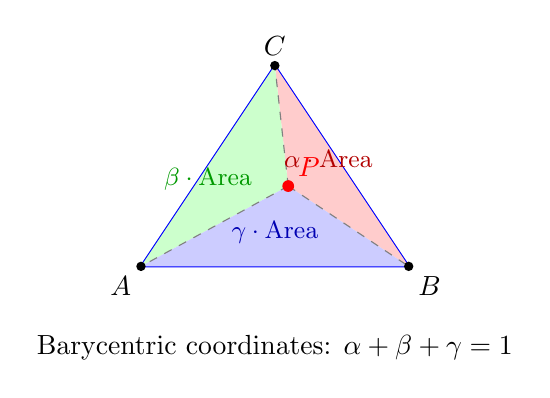
\begin{tikzpicture}[scale=0.85]
    % Source triangle
    \coordinate (A) at (0,0);
    \coordinate (B) at (4,0);
    \coordinate (C) at (2,3);

    % Point P inside
    \coordinate (P) at (2.2,1.2);

    % Draw triangle
    \draw[thick, blue] (A) -- (B) -- (C) -- cycle;

    % Fill sub-triangles with different opacities
    \fill[red!20]   (P) -- (B) -- (C) -- cycle;
    \fill[green!20] (P) -- (C) -- (A) -- cycle;
    \fill[blue!20]  (P) -- (A) -- (B) -- cycle;

    % Draw lines from P to vertices
    \draw[dashed, gray] (P) -- (A);
    \draw[dashed, gray] (P) -- (B);
    \draw[dashed, gray] (P) -- (C);

    % Labels
    \fill[black] (A) circle (2pt) node[below left] {$A$};
    \fill[black] (B) circle (2pt) node[below right] {$B$};
    \fill[black] (C) circle (2pt) node[above] {$C$};
    \fill[red] (P) circle (2.5pt) node[above right] {$P$};

    % Area labels
    \node[red!70!black, font=\small] at (2.8,1.6) {$\alpha \cdot \operatorname{Area}$};
    \node[green!60!black, font=\small] at (1.0,1.3) {$\beta \cdot \operatorname{Area}$};
    \node[blue!70!black, font=\small] at (2.0,0.5) {$\gamma \cdot \operatorname{Area}$};

    \node[below=0.5cm] at (2,-0.3) {Barycentric coordinates: $\alpha+\beta+\gamma=1$};
\end{tikzpicture}
\caption{Barycentric coordinates of point $P$ with respect to triangle $ABC$.  Each coordinate equals the area of the opposite sub-triangle divided by the total area.}
\label{fig:barycentric}
\end{figure}

%-----------------------------------------------------------------------
\subsection{Inverse Mapping vs.~Forward Mapping}
%-----------------------------------------------------------------------

Once we can map the vertices of each triangle, we must decide \emph{how} to transfer pixel values.  There are two fundamentally different approaches.

\paragraph{Forward mapping.}
For each pixel $(x, y)$ in the source image, compute its destination $(x', y') = \mathbf{T}(x, y)$.  This \emph{sounds} natural, but it has a critical flaw: because the transform is not in general integer-preserving, many destination pixels will \emph{never be hit} (they fall between mapped source pixels), producing visible \textbf{holes} in the output.  Rounding to nearest integer mitigates but does not eliminate the problem.

\begin{figure}[htbp]
\centering
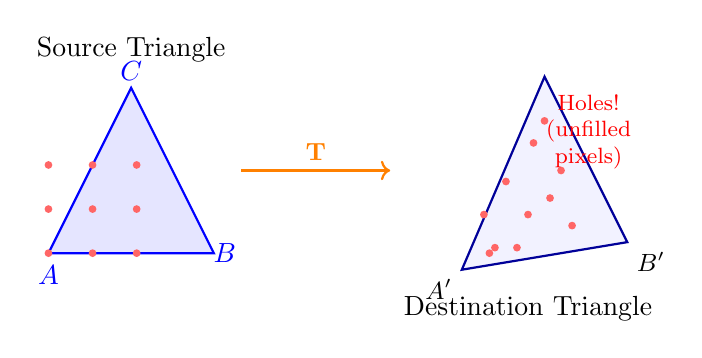
\begin{tikzpicture}[scale=0.7]
    % ---- Source triangle ----
    \begin{scope}[xshift=-5cm]
        \coordinate (A) at (0,0);
        \coordinate (B) at (3,0);
        \coordinate (C) at (1.5,3);

        \draw[thick, blue, fill=blue!10] (A) -- (B) -- (C) -- cycle;

        % Source pixel grid
        \foreach \i in {0,1,2} {
            \foreach \j in {0,1,2} {
                \coordinate (pixel\i\j) at (\i*0.8, \j*0.8);
                \fill[red!60] (pixel\i\j) circle (2pt);
            }
        }

        % Labels
        \node[above] at (1.5,3.3) {Source Triangle};
        \node[blue] at (0,-0.4) {$A$};
        \node[blue] at (3.2,0) {$B$};
        \node[blue] at (1.5,3.3) {$C$};
    \end{scope}

    % Arrow
    \draw[->, thick, orange] (-1.5,1.5) -- (1.2,1.5)
        node[midway, above, font=\small] {$\mathbf{T}$};

    % ---- Destination triangle ----
    \begin{scope}[xshift=2cm]
        \coordinate (A') at (0.5,-0.3);
        \coordinate (B') at (3.5,0.2);
        \coordinate (C') at (2,3.2);

        \draw[thick, blue!60!black, fill=blue!5] (A') -- (B') -- (C') -- cycle;

        % Mapped pixels (sparse, with gaps)
        \fill[red!60] (1.1,0.1)  circle (2pt);
        \fill[red!60] (1.5,0.1)  circle (2pt);
        \fill[red!60] (0.9,0.7)  circle (2pt);
        \fill[red!60] (1.7,0.7)  circle (2pt);
        \fill[red!60] (1.3,1.3)  circle (2pt);
        \fill[red!60] (2.1,1.0)  circle (2pt);
        \fill[red!60] (2.5,0.5)  circle (2pt);
        \fill[red!60] (1.0,0.0)  circle (2pt);
        \fill[red!60] (2.3,1.5)  circle (2pt);
        \fill[red!60] (1.8,2.0)  circle (2pt);
        \fill[red!60] (2.0,2.4)  circle (2pt);

        % Label gaps
        \node[red, font=\footnotesize, align=center] at (2.8,2.2) {Holes!\\(unfilled\\pixels)};

        \node[below] at (1.7,-0.6) {Destination Triangle};
        \node at (A') [below left, font=\small] {$A'$};
        \node at (B') [below right, font=\small] {$B'$};
    \end{scope}
\end{tikzpicture}
\caption{Forward mapping sends discrete source pixels to the destination, leaving gaps (holes).  Not all destination pixels receive a value.}
\label{fig:forward-mapping}
\end{figure}

\paragraph{Inverse mapping.}
Instead of asking ``where does each source pixel go?'', we ask ``where did each destination pixel come from?''.  Concretely, for each pixel $(x', y')$ in the destination, we compute
\[
    \begin{bmatrix} x \\ y \\ 1 \end{bmatrix}
    = \mathbf{T}^{-1}
    \begin{bmatrix} x' \\ y' \\ 1 \end{bmatrix},
\]
where $\mathbf{T}^{-1}$ is the inverse of the affine transform matrix.  We then sample the source image at the (generally non-integer) position $(x, y)$ using interpolation (nearest-neighbor, bilinear, or bicubic).

\paragraph{Why inverse mapping wins.}
\begin{itemize}
    \item \textbf{No holes:} every destination pixel is visited exactly once, so the output is complete.
    \item \textbf{Parallelizable:} each destination pixel can be processed independently.
    \item \textbf{Well-defined:} the only remaining design choice is the interpolation kernel at non-integer source locations.
\end{itemize}

The inverse of a homogeneous affine matrix
\[
    \mathbf{T} =
    \begin{bmatrix}
        \mathbf{A} & \mathbf{t} \\
        \mathbf{0}^\top & 1
    \end{bmatrix}
\]
has the closed form
\[
    \mathbf{T}^{-1} =
    \begin{bmatrix}
        \mathbf{A}^{-1} & -\mathbf{A}^{-1}\mathbf{t} \\
        \mathbf{0}^\top & 1
    \end{bmatrix},
\]
where $\mathbf{A}^{-1} = \frac{1}{\det(\mathbf{A})}
\begin{bmatrix}
    a_{22} & -a_{12} \\
    -a_{21} & a_{11}
\end{bmatrix}$.

\paragraph{Putting it all together.}\label{sec:inverse-mapping}
The complete inverse-mapping warp for a single triangle pair is:
\begin{enumerate}
    \item Compute $\mathbf{T}$ from the three vertex correspondences (Section~2).
    \item Invert $\mathbf{T}$ to obtain $\mathbf{T}^{-1}$.
    \item For each pixel $(x', y')$ in the bounding box of the destination triangle:
    \begin{enumerate}
        \item Compute barycentric coordinates of $(x', y')$ w.r.t.\ the destination triangle.
        \item If any coordinate is negative, the pixel is outside the triangle --- skip it.
        \item Otherwise, apply $\mathbf{T}^{-1}$ to find the corresponding source location $(x, y)$.
        \item Sample the source image at $(x, y)$ by interpolation and write the value to the output.
    \end{enumerate}
\end{enumerate}

This algorithm is fast, exact, and guaranteed to produce a complete output image with no holes.  In the next section we will see how to choose the triangulation that drives all of these individual triangle warps.

\section{Delaunay Triangulation}

\subsection{What Is a Triangulation?}

Given a set of distinct points $P = \{p_1, p_2, \dots, p_N\}$ in the plane $\mathbb{R}^2$,
a \emph{triangulation} is a subdivision of the convex hull of $P$ into triangles such that:
\begin{itemize}
    \item every triangle vertex is a point from $P$,
    \item the interiors of any two triangles do not intersect,
    \item the union of all triangles equals the convex hull of $P$.
\end{itemize}

In other words, a triangulation connects the given points with non-crossing edges
to form a tiling of triangles covering the entire convex hull, leaving no gaps
or overlaps.  A single point set typically admits many different triangulations.
Figure~\ref{fig:triang-comparison} shows two valid triangulations of the same
point set---they use identical vertices but different edge connections.

\begin{figure}[htbp]
    \centering
    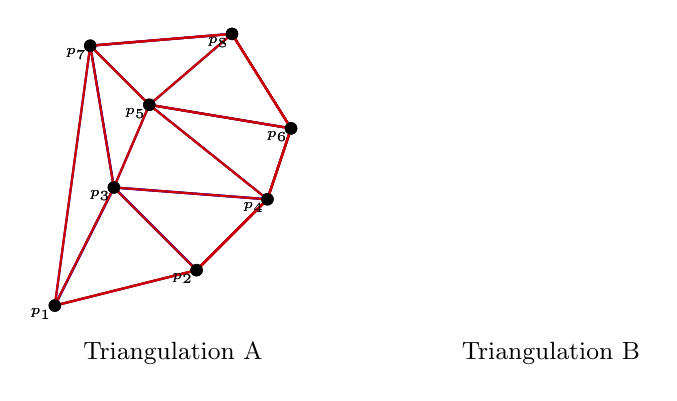
\begin{tikzpicture}[scale=1.5]
        % Point positions
        \coordinate (A) at (0, 0);
        \coordinate (B) at (1.2, 0.3);
        \coordinate (C) at (0.5, 1.0);
        \coordinate (D) at (1.8, 0.9);
        \coordinate (E) at (0.8, 1.7);
        \coordinate (F) at (2.0, 1.5);
        \coordinate (G) at (0.3, 2.2);
        \coordinate (H) at (1.5, 2.3);

        % --- Left: Triangulation 1 ---
        \begin{scope}[xshift=0cm]
            \draw[gray!60, thin] (A) -- (B) -- (D) -- (F) -- (H) -- (G) -- cycle;
            \draw[blue!80!black, thick] (A) -- (B) -- (D) -- (F) -- (H) -- (G) -- cycle;
            \draw[blue!80!black, thick] (A) -- (C) -- (B);
            \draw[blue!80!black, thick] (A) -- (C) -- (G);
            \draw[blue!80!black, thick] (B) -- (C) -- (E);
            \draw[blue!80!black, thick] (B) -- (D) -- (C);
            \draw[blue!80!black, thick] (C) -- (D) -- (E);
            \draw[blue!80!black, thick] (C) -- (G) -- (E);
            \draw[blue!80!black, thick] (D) -- (F) -- (E);
            \draw[blue!80!black, thick] (E) -- (F) -- (H);
            \draw[blue!80!black, thick] (E) -- (H) -- (G);

            \foreach \pt/\lbl in {A/$p_1$,B/$p_2$,C/$p_3$,D/$p_4$,E/$p_5$,F/$p_6$,G/$p_7$,H/$p_8$}
            {
                \fill[black] (\pt) circle (1.5pt);
                \node[anchor=north east, font=\tiny, inner sep=1pt] at (\pt) {\lbl};
            }
            \node at (1.0, -0.4) {\small Triangulation A};
        \end{scope}

        % --- Right: Triangulation 2 ---
        \begin{scope}[xshift=3.2cm]
            \draw[gray!60, thin] (A) -- (B) -- (D) -- (F) -- (H) -- (G) -- cycle;
            \draw[red!80!black, thick] (A) -- (B) -- (D) -- (F) -- (H) -- (G) -- cycle;
            \draw[red!80!black, thick] (A) -- (C) -- (G);
            \draw[red!80!black, thick] (A) -- (B) -- (C);
            \draw[red!80!black, thick] (B) -- (D) -- (C);
            \draw[red!80!black, thick] (B) -- (D) -- (E);
            \draw[red!80!black, thick] (C) -- (E) -- (G);
            \draw[red!80!black, thick] (D) -- (F) -- (E);
            \draw[red!80!black, thick] (D) -- (F) -- (H);
            \draw[red!80!black, thick] (E) -- (F) -- (H);
            \draw[red!80!black, thick] (E) -- (H) -- (G);

            \foreach \pt/\lbl in {A/$p_1$,B/$p_2$,C/$p_3$,D/$p_4$,E/$p_5$,F/$p_6$,G/$p_7$,H/$p_8$}
            {
                \fill[black] (\pt) circle (1.5pt);
                \node[anchor=north east, font=\tiny, inner sep=1pt] at (\pt) {\lbl};
            }
            \node at (1.0, -0.4) {\small Triangulation B};
        \end{scope}
    \end{tikzpicture}
    \caption{Two different valid triangulations of the same eight-point set.
    The convex hull edges (darker) are the same in both, but the internal
    edges differ, yielding different triangle shapes and qualities.}
    \label{fig:triang-comparison}
\end{figure}

For $N$ points in \emph{general position} (no three collinear), the number of
triangles and edges in any triangulation is fixed.  If $h$ of the $N$ points lie
on the convex hull boundary, then every triangulation has exactly
\[
    T = 2N - 2 - h \quad \text{triangles}
    \qquad\text{and}\qquad
    E = 3N - 3 - h \quad \text{edges}.
\]
When the points are well distributed (roughly $h \approx \sqrt{N}$), this is
approximately $2N$ triangles and $3N$ edges.  The counting follows from Euler's
formula for planar graphs: $V - E + F = 1 + C$, where for a triangulation
$V = N$, each internal face is a triangle, and $C = 1$ for a connected graph.

\subsection{Why Triangulation in Face Morphing?}

In feature-based face morphing, we place landmark points on key facial features
(eyes, nose, mouth contour, jawline, etc.) in both source and target images.
The next step is \emph{warping}: moving pixels from the source image to their
corresponding positions in the target.  Triangulation provides the geometric
framework for this warp.

Each triangle in the source triangulation maps to a corresponding triangle in
the target triangulation via an \emph{affine transformation}.  Affine transforms
preserve lines and ratios of distances, so lines inside a triangle remain lines
after warping---a critical property for avoiding visible seams.

Triangles are the ideal choice for several reasons:
\begin{enumerate}
    \item \textbf{Uniqueness of the transform.} Three non-collinear points
    uniquely determine an affine transformation.  Given source triangle
    $(a, b, c)$ and target triangle $(a', b', c')$, there is exactly one
    affine map $T$ with $T(a)=a'$, $T(b)=b'$, $T(c)=c'$.
    \item \textbf{Planarity.} A triangle is always planar---its three vertices
    always lie in a single plane.  Under an affine transformation, the image of
    a triangle is always another triangle, never a self-intersecting shape.
    \item \textbf{Complete partitioning.} A triangulation covers the convex hull
    entirely, with no gaps between triangles and no overlaps (except shared
    edges).  Every pixel inside the hull belongs to exactly one triangle.
    \item \textbf{Why not quadrilaterals or higher polygons?} A quadrilateral
    is not necessarily planar under an affine transform---its four vertices may
    map to a non-planar configuration that cannot be represented by a single
    affine map in 2D.  One could subdivide a quadrilateral into two triangles,
    but then we are back to triangulation.  Higher-order polygons have the same
    problem, worsened.
\end{enumerate}

The quality of the triangulation directly affects the visual quality of the
morph.  Long, thin (``skinny'') triangles produce highly non-uniform stretches
that look visibly distorted.  This motivates choosing a triangulation that
avoids skinny triangles---which brings us to the Delaunay triangulation.

\subsection{The Delaunay Triangulation}

\begin{definition}[Circumcircle]
    The \emph{circumcircle} of a triangle is the unique circle passing through
    all three of its vertices.  Every non-degenerate triangle has exactly one
    circumcircle.  The center of the circumcircle (the \emph{circumcenter}) is
    the intersection of the three perpendicular bisectors of the triangle's edges.
\end{definition}

\begin{theorem}[Empty Circumcircle Property]
    Given a set of points $P \subset \mathbb{R}^2$, the \emph{Delaunay
    triangulation} $DT(P)$ is the unique triangulation of $P$ satisfying the
    following property: for every triangle $\triangle abc$ in $DT(P)$, the open
    interior of its circumcircle contains no point of $P$.
\end{theorem}

Equivalently, no point of $P$ lies strictly inside the circumcircle of any
triangle in the Delaunay triangulation.  Points may lie \emph{on} the
circumcircle (this happens precisely when four or more points are co-circular),
but never strictly inside.

\begin{figure}[htbp]
    \centering
    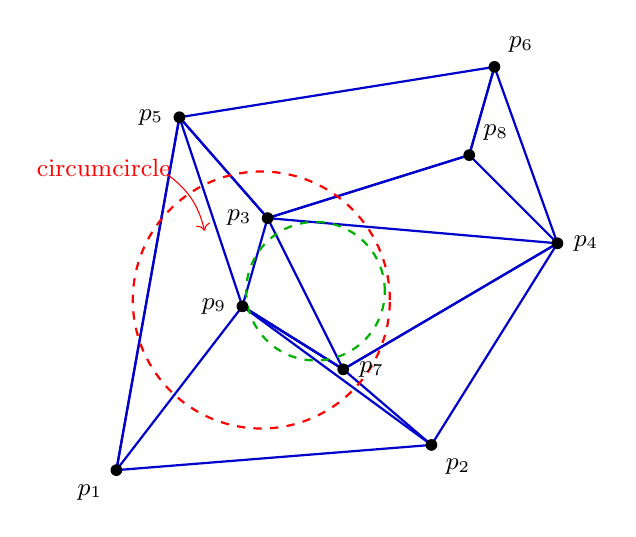
\begin{tikzpicture}[scale=1.6]
        % Define points
        \coordinate (A) at (0, 0);
        \coordinate (B) at (2.5, 0.2);
        \coordinate (C) at (1.2, 2.0);
        \coordinate (D) at (3.5, 1.8);
        \coordinate (E) at (0.5, 2.8);
        \coordinate (F) at (3.0, 3.2);
        \coordinate (G) at (1.8, 0.8);
        \coordinate (H) at (2.8, 2.5);
        \coordinate (I) at (1.0, 1.3);

        % Delaunay triangulation edges
        \draw[blue!80!black, thick] (A) -- (B) -- (D) -- (F) -- (E) -- cycle;
        \draw[blue!80!black, thick] (A) -- (I) -- (B);
        \draw[blue!80!black, thick] (A) -- (E) -- (I);
        \draw[blue!80!black, thick] (I) -- (G) -- (B);
        \draw[blue!80!black, thick] (I) -- (G) -- (D);
        \draw[blue!80!black, thick] (I) -- (G) -- (C);
        \draw[blue!80!black, thick] (I) -- (C) -- (E);
        \draw[blue!80!black, thick] (G) -- (D) -- (C);
        \draw[blue!80!black, thick] (C) -- (H) -- (D);
        \draw[blue!80!black, thick] (C) -- (H) -- (F);
        \draw[blue!80!black, thick] (C) -- (E);
        \draw[blue!80!black, thick] (H) -- (F);

        % Highlight one triangle with circumcircle
        \coordinate (O1) at (1.15, 1.35); % approximate circumcenter of A, I, E
        \pgfmathsetmacro{\rOne}{1.02}

        \draw[red, dashed, thick] (O1) circle (\rOne);

        % Circumcircle of I, G, C
        \coordinate (O2) at (1.58, 1.42);
        \pgfmathsetmacro{\rTwo}{0.55}
        \draw[green!70!black, dashed, thick] (O2) circle (\rTwo);

        % Points
        \foreach \pt/\lbl/\pos in {
            A/$p_1$/below left,
            B/$p_2$/below right,
            C/$p_3$/left,
            D/$p_4$/right,
            E/$p_5$/left,
            F/$p_6$/above right,
            G/$p_7$/right,
            H/$p_8$/above right,
            I/$p_9$/left
        } {
            \node[circle, fill=black, inner sep=1.5pt, label={\pos:\small\lbl}] at (\pt) {};
        }

        % Label highlighting circumcircle
        \node[red, font=\small] at (-0.1, 2.4) {circumcircle};
        \draw[red, ->] (0.4, 2.35) to [bend left=20] (0.7, 1.9);
    \end{tikzpicture}
    \caption{Delaunay triangulation of a nine-point set.  The red dashed circle
    is the circumcircle of one triangle; notice that no other points lie
    strictly inside it.  This is the defining \emph{empty circumcircle property}
    of the Delaunay triangulation.}
    \label{fig:delaunay-circumcircle}
\end{figure}

\paragraph{Connection to the Voronoi Diagram.}
The Delaunay triangulation is closely related to the Voronoi diagram.
Given $P = \{p_1, \dots, p_N\}$, the Voronoi cell of $p_i$ is the region of
the plane consisting of all points closer to $p_i$ than to any other point:
\[
    V(p_i) = \{\, x \in \mathbb{R}^2 \mid \|x - p_i\| \leq \|x - p_j\|
    \text{ for all } j \neq i \,\}.
\]
The \emph{Voronoi diagram} is the subdivision of the plane into these cells.
The Delaunay triangulation is the \emph{dual graph} of the Voronoi diagram:
two points $p_i$ and $p_j$ are connected by a Delaunay edge if and only if
their Voronoi cells $V(p_i)$ and $V(p_j)$ share a boundary segment.  This
duality provides both geometric intuition and practical algorithms: computing
the Voronoi diagram immediately yields the Delaunay triangulation and vice versa.

\subsection{Key Properties of Delaunay Triangulation}

The Delaunay triangulation is preferred over arbitrary triangulations because
of several optimality properties.

\subsubsection*{Max--Min Angle Property}

\begin{theorem}[Max--Min Angle]
    Among all possible triangulations of a given point set, the Delaunay
    triangulation maximizes the minimum interior angle across all triangles.
    That is, if $\alpha_{\min}(T)$ denotes the smallest interior angle in
    triangulation $T$, then
    \[
        \alpha_{\min}(DT(P)) \geq \alpha_{\min}(T)
        \quad \text{for all triangulations } T \text{ of } P.
    \]
\end{theorem}

This property is crucial for face morphing.  Triangles with very small angles
are ``skinny''---they have a large aspect ratio.  When a skinny triangle is
affinely mapped to a better-shaped target triangle, the mapping stretches
pixels enormously in one direction and compresses them in another, producing
visible artifacts.  The max--min angle guarantee ensures that Delaunay
triangles are as ``equilateral as possible,'' minimizing distortion.

\subsubsection*{Uniqueness}

\begin{proposition}
    If no four points of $P$ lie on a common circle (the \emph{general
    position} assumption), then the Delaunay triangulation of $P$ is unique.
\end{proposition}

When four or more points are co-circular, there can be multiple valid Delaunay
triangulations.  For example, four points forming a rectangle all lie on a
common circle; the diagonal can be chosen either way and both triangulations
satisfy the empty circumcircle property.  In practice with real-valued landmark
coordinates, co-circularity is extremely unlikely.

\subsubsection*{Local (Incremental) Property}

An important practical property is that the Delaunay triangulation can be
constructed incrementally.  Given $DT(\{p_1, \dots, p_k\})$, inserting a new
point $p_{k+1}$ requires modifying only the triangles whose circumcircles
contain $p_{k+1}$.  All other triangles remain unchanged.  This is the key
insight behind many efficient Delaunay construction algorithms.

\subsection{The Bowyer--Watson Algorithm}

The Bowyer--Watson algorithm is an incremental algorithm for constructing the
Delaunay triangulation.  It was published independently by Bowyer (1981) and
Watson (1981), and is widely used in practice due to its simplicity and
robustness.

\subsubsection*{Algorithm Steps}

\begin{enumerate}
    \item \textbf{Create a super-triangle.} Start with an artificial triangle
    large enough to contain all input points.  This avoids boundary-condition
    complications during incremental insertion.
    \item \textbf{Insert points one at a time.} For each point $p$:
    \begin{enumerate}
        \item \textbf{Find bad triangles.} Identify all existing triangles
        whose circumcircles contain $p$.  These triangles violate the empty
        circumcircle property and must be removed.
        \item \textbf{Find the cavity boundary.} The removed triangles create
        a polygonal hole (the \emph{cavity}).  Find the unique polygon edges
        on the boundary of this hole---edges that belong to exactly one removed
        triangle (the other side is part of the hole interior).
        \item \textbf{Re-triangulate.} Connect $p$ to each vertex of the
        cavity boundary, forming new triangles.  Each new triangle has $p$ as
        one vertex and a cavity boundary edge as the opposite side.
    \end{enumerate}
    \item \textbf{Remove super-triangle artifacts.} After all points have been
    inserted, discard any triangle that shares a vertex with the original
    super-triangle.
\end{enumerate}

\begin{figure}[htbp]
    \centering
    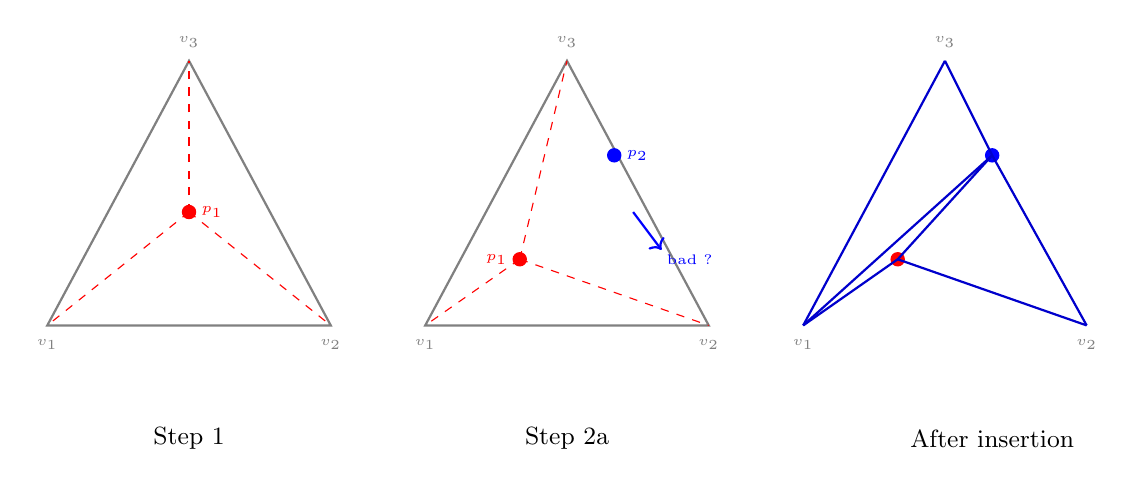
\begin{tikzpicture}[scale=1.2]
        % Step 1: Super-triangle with one point
        \begin{scope}[xshift=0cm]
            \node[font=\small] at (1.5, -1.2) {Step 1};
            \draw[gray, thick] (0, 0) -- (3, 0) -- (1.5, 2.8) -- cycle;
            \node[gray, font=\tiny] at (0, -0.2) {$v_1$};
            \node[gray, font=\tiny] at (3, -0.2) {$v_2$};
            \node[gray, font=\tiny] at (1.5, 3.0) {$v_3$};
            \filldraw[red] (1.5, 1.2) circle (2pt) node[right=1pt] {\tiny $p_1$};
            \draw[red, dashed] (1.5, 1.2) -- (0, 0);
            \draw[red, dashed] (1.5, 1.2) -- (3, 0);
            \draw[red, dashed] (1.5, 1.2) -- (1.5, 2.8);
        \end{scope}

        % Step 2: Add second point, find bad triangle
        \begin{scope}[xshift=4cm]
            \node[font=\small] at (1.5, -1.2) {Step 2a};
            \draw[gray, thick] (0, 0) -- (3, 0) -- (1.5, 2.8) -- cycle;
            \node[gray, font=\tiny] at (0, -0.2) {$v_1$};
            \node[gray, font=\tiny] at (3, -0.2) {$v_2$};
            \node[gray, font=\tiny] at (1.5, 3.0) {$v_3$};
            \filldraw[red] (1.0, 0.7) circle (2pt) node[left=1pt] {\tiny $p_1$};
            \filldraw[blue] (2.0, 1.8) circle (2pt) node[right=1pt] {\tiny $p_2$};

            \draw[red, dashed] (1.0, 0.7) -- (0, 0);
            \draw[red, dashed] (1.0, 0.7) -- (3, 0);
            \draw[red, dashed] (1.0, 0.7) -- (1.5, 2.8);

            \draw[blue, ->, thick] (2.2, 1.2) -- (2.5, 0.8);
            \node[blue, font=\tiny] at (2.8, 0.7) {bad ?};
        \end{scope}

        % Step 3: After insertion
        \begin{scope}[xshift=8cm]
            \node[font=\small] at (2.0, -1.2) {After insertion};
            \filldraw[red] (1.0, 0.7) circle (2pt);
            \filldraw[blue] (2.0, 1.8) circle (2pt);
            \draw[blue!80!black, thick] (0, 0) -- (1.0, 0.7);
            \draw[blue!80!black, thick] (3, 0) -- (1.0, 0.7);
            \draw[blue!80!black, thick] (1.0, 0.7) -- (2.0, 1.8);
            \draw[blue!80!black, thick] (2.0, 1.8) -- (0, 0);
            \draw[blue!80!black, thick] (2.0, 1.8) -- (3, 0);
            \draw[blue!80!black, thick] (1.5, 2.8) -- (0, 0);
            \draw[blue!80!black, thick] (1.5, 2.8) -- (2.0, 1.8);
            \node[gray, font=\tiny] at (0, -0.2) {$v_1$};
            \node[gray, font=\tiny] at (3, -0.2) {$v_2$};
            \node[gray, font=\tiny] at (1.5, 3.0) {$v_3$};
        \end{scope}
    \end{tikzpicture}
    \caption{Illustration of the Bowyer--Watson algorithm inserting two points
    into a super-triangle.  Each new point identifies the triangles whose
    circumcircles contain it, removes them, and re-triangulates the cavity.}
    \label{fig:bowyer-watson}
\end{figure}

\subsubsection*{Pseudocode}

\begin{algorithm}[H]
\caption{Bowyer--Watson Delaunay Triangulation}
\label{alg:bowyer-watson}
\begin{algorithmic}[1]
\Require A set of points $P = \{p_1, p_2, \dots, p_N\}$
\Ensure Delaunay triangulation $DT(P)$
\State Create a super-triangle $T_{\text{super}}$ containing all points in $P$
\State $\mathcal{T} \gets \{T_{\text{super}}\}$ \Comment{current triangulation}
\For{each point $p \in P$}
    \State $\mathcal{B} \gets \emptyset$ \Comment{bad triangles}
    \For{each triangle $t \in \mathcal{T}$}
        \If{$p$ is inside the circumcircle of $t$}
            \State $\mathcal{B} \gets \mathcal{B} \cup \{t\}$
        \EndIf
    \EndFor
    \State $\mathcal{E}_{\text{boundary}} \gets \emptyset$ \Comment{cavity boundary edges}
    \For{each triangle $t \in \mathcal{B}$}
        \For{each edge $e$ of $t$}
            \If{$e$ is not shared with another triangle in $\mathcal{B}$}
                \State $\mathcal{E}_{\text{boundary}} \gets \mathcal{E}_{\text{boundary}} \cup \{e\}$
            \EndIf
        \EndFor
    \EndFor
    \State $\mathcal{T} \gets \mathcal{T} \setminus \mathcal{B}$
    \For{each edge $(v_i, v_j) \in \mathcal{E}_{\text{boundary}}$}
        \State $\mathcal{T} \gets \mathcal{T} \cup \{\triangle(v_i, v_j, p)\}$
    \EndFor
\EndFor
\State Remove all triangles from $\mathcal{T}$ that share a vertex with $T_{\text{super}}$
\State \Return $\mathcal{T}$
\end{algorithmic}
\end{algorithm}

\subsubsection*{Complexity}

The naive implementation has worst-case time complexity $O(N^2)$: for each
of the $N$ points, we may check all $O(N)$ existing triangles, and the number
of bad triangles per insertion is $O(N)$ in the worst case.  With spatial
indexing structures (such as a quadtree or walk-based point location), the
complexity can be reduced to $O(N \log N)$ for uniformly distributed points.
The space complexity is $O(N)$ since the triangulation always has $O(N)$
triangles and edges.

\begin{remark}
    In practice, for face morphing applications, the number of landmark points
    is typically between 50 and 200, so even the naive $O(N^2)$ implementation
    runs nearly instantaneously.  The Bowyer--Watson algorithm's simplicity and
    robustness make it an excellent choice for this use case.
\end{remark}

\subsection{OpenCV Implementation}

OpenCV provides a convenient 2D subdivision class \texttt{cv2.Subdiv2D} that
implements an incremental Delaunay triangulation.  The typical workflow is:

\begin{enumerate}
    \item Create a \texttt{Subdiv2D} object initialized with the bounding
    rectangle of your image.
    \item Insert each landmark point using \texttt{insert()}.
    \item Extract the resulting triangles using \texttt{getTriangleList()}.
\end{enumerate}

Here is a minimal working example:

\begin{minted}[linenos, fontsize=\small, breaklines]{python}
import cv2
import numpy as np

def delaunay_triangulation(points, img_width, img_height):
    """Compute Delaunay triangulation of landmark points.

    Args:
        points: numpy array of shape (N, 2) with landmark coordinates.
        img_width:  width of the image bounding box.
        img_height: height of the image bounding box.

    Returns:
        List of triangles, each a triplet of point indices.
    """
    # Step 1: create subdiv with the image rectangle
    rect = (0, 0, img_width, img_height)
    subdiv = cv2.Subdiv2D(rect)

    # Step 2: convert points to (x, y) tuples and insert
    for pt in points:
        subdiv.insert((float(pt[0]), float(pt[1])))

    # Step 3: extract triangles
    triangle_list = subdiv.getTriangleList()
    # Each row is [x1, y1, x2, y2, x3, y3]

    # Step 4: map each triangle vertex back to point indices
    triangles = []
    for tri in triangle_list:
        p1 = (tri[0], tri[1])
        p2 = (tri[2], tri[3])
        p3 = (tri[4], tri[5])
        idx1 = find_point_index(points, p1)
        idx2 = find_point_index(points, p2)
        idx3 = find_point_index(points, p3)
        if idx1 >= 0 and idx2 >= 0 and idx3 >= 0:
            triangles.append((idx1, idx2, idx3))

    return triangles
\end{minted}

\begin{remark}[Practical note]
    The \texttt{Subdiv2D} class internally handles its own super-triangle and
    clipping region.  Points outside the bounding rectangle are silently
    rejected, so the rectangle should be chosen to contain all landmarks.
    For full-image face morphing, use the image dimensions as the bounding
    rectangle.
\end{remark}

The triangles returned by \texttt{getTriangleList()} are expressed in
coordinates, not as indices into the original point set.  In practice, one
matches each triangle vertex to the nearest landmark point (typically by
Euclidean distance with a small tolerance) to build the index-based triangle
list needed for warping.

\section{Piecewise Affine Warping}

In the previous sections we established the mathematical and geometric prerequisites for feature-based face morphing: we can detect and align facial landmarks, we understand how to decompose a face into a Delaunay triangulation, and we know how to compute affine transformations and barycentric coordinates. In this section we combine all of these ingredients into the core rendering engine of the morphing pipeline: \textbf{piecewise affine warping}.

\subsection{The Concept}

The central idea is conceptually simple but computationally powerful. Once we have:
\begin{enumerate}
    \item A set of corresponding landmarks on Face~A and Face~B,
    \item A Delaunay triangulation computed on a \emph{mean shape} (defined below),
    \item The theory to compute an affine transform between any two corresponding triangles,
\end{enumerate}
we can \emph{warp} each input face into a common geometric frame.

For every triangle in the mean-shape mesh, we compute two independent affine transforms: one that maps the corresponding triangle in Face~A to the mean triangle, and another that maps the corresponding triangle in Face~B to the mean triangle. Applying these transforms pixel-by-pixel renders both faces so that their facial features (eyes, nose, mouth, jawline) are perfectly aligned to the intermediate geometry. Because affine transformations are linear, they preserve straight lines along triangle edges, which guarantees that adjacent triangles meet seamlessly without visible seams or discontinuities. This is why the method is called \emph{piecewise} affine: globally non-rigid, but locally affine within each triangle.

\begin{figure}[h]
\centering
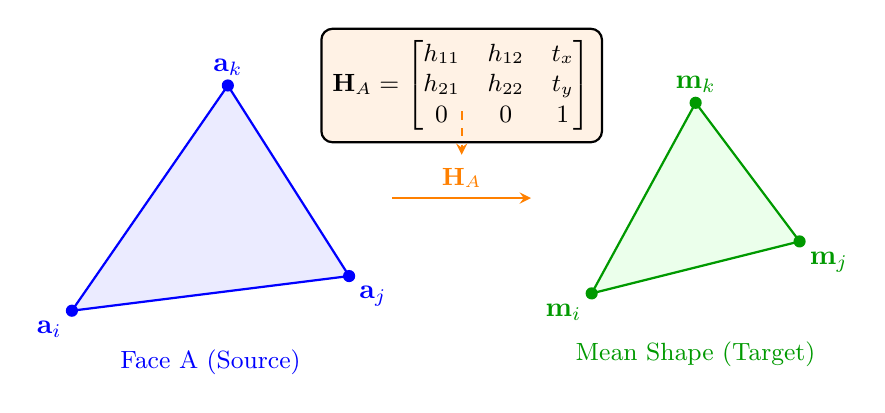
\begin{tikzpicture}[>=stealth, line width=0.8pt, scale=1.1]
    % Source Triangle
    \coordinate (A1) at (0,0);
    \coordinate (A2) at (3.2,0.4);
    \coordinate (A3) at (1.8,2.6);
    \draw[thick, blue, fill=blue!8] (A1) -- (A2) -- (A3) -- cycle;
    \fill[blue] (A1) circle (2pt) node[below left] {$\mathbf{a}_i$};
    \fill[blue] (A2) circle (2pt) node[below right] {$\mathbf{a}_j$};
    \fill[blue] (A3) circle (2pt) node[above] {$\mathbf{a}_k$};
    \node[blue, font=\small] at (1.6, -0.6) {Face~A (Source)};

    % Arrow
    \draw[->, thick, orange] (3.7, 1.3) -- node[above, pos=0.5, sloped] {\small $\mathbf{H}_A$} (5.3, 1.3);

    % Mean Triangle
    \coordinate (M1) at (6, 0.2);
    \coordinate (M2) at (8.4, 0.8);
    \coordinate (M3) at (7.2, 2.4);
    \draw[thick, green!60!black, fill=green!8] (M1) -- (M2) -- (M3) -- cycle;
    \fill[green!60!black] (M1) circle (2pt) node[below left] {$\mathbf{m}_i$};
    \fill[green!60!black] (M2) circle (2pt) node[below right] {$\mathbf{m}_j$};
    \fill[green!60!black] (M3) circle (2pt) node[above] {$\mathbf{m}_k$};
    \node[green!60!black, font=\small] at (7.2, -0.5) {Mean Shape (Target)};

    % Matrix box
    \node[draw, rounded corners, fill=orange!10, inner sep=4pt, font=\small] at (4.5, 2.6) {
        $\mathbf{H}_A = \begin{bmatrix}
            h_{11} & h_{12} & t_x \\
            h_{21} & h_{22} & t_y \\
            0 & 0 & 1
        \end{bmatrix}$
    };
    \draw[->, orange, dashed] (4.5, 2.3) -- (4.5, 1.8);
\end{tikzpicture}
\caption{Single-triangle affine warp. Three landmark correspondences determine a unique $3 \times 3$ homogeneous matrix $\mathbf{H}_A$ that maps the source triangle in Face~A to the corresponding triangle in the mean shape. The top two rows of $\mathbf{H}_A$ form the standard $2 \times 3$ affine warp matrix used in image processing.}
\label{fig:single-triangle-warp}
\end{figure}

\subsection{Computing the Mean Shape}

The first step is to define the common target geometry. Given two sets of corresponding landmarks
\[
    L_A = \{\mathbf{a}_1, \mathbf{a}_2, \ldots, \mathbf{a}_n\}, \quad
    L_B = \{\mathbf{b}_1, \mathbf{b}_2, \ldots, \mathbf{b}_n\},
\]
where each $\mathbf{a}_i, \mathbf{b}_i \in \mathbb{R}^2$ are 2D image coordinates, the \emph{mean shape} is simply the arithmetic average of corresponding points:
\begin{equation}
    \mathbf{m}_i = \frac{\mathbf{a}_i + \mathbf{b}_i}{2}, \quad i = 1, \ldots, n.
\end{equation}
The complete mean landmark set is $M = \{\mathbf{m}_1, \ldots, \mathbf{m}_n\}$. This symmetric average places the target geometry exactly halfway between the two faces, which is ideal for a 50/50 morph.

More generally, one can define a \emph{weighted} mean shape:
\begin{equation}
    \mathbf{m}_i(\alpha) = (1 - \alpha)\,\mathbf{a}_i + \alpha\,\mathbf{b}_i, \quad \alpha \in [0, 1],
\end{equation}
where $\alpha = 0$ yields the original Face~A geometry, $\alpha = 1$ yields Face~B, and $\alpha = 0.5$ recovers the simple average. In a full morphing pipeline, $\alpha$ is varied smoothly from 0 to 1 to produce the intermediate frames of the animation.

\subsection{The Triangular Correspondence}

Once the mean landmarks $M$ are computed, we run Delaunay triangulation on them. The triangulation yields a set of triangles
\[
    \mathcal{T}_{\text{mean}} = \{ T_{\text{mean}}^{(1)}, T_{\text{mean}}^{(2)}, \ldots, T_{\text{mean}}^{(K)} \},
\]
where each triangle is defined by three vertex indices: $T_{\text{mean}}^{(p)} = (\mathbf{m}_i, \mathbf{m}_j, \mathbf{m}_k)$.

Because the triangulation is computed on the \emph{indices} of the landmarks, the same index triplet automatically defines corresponding triangles in the source faces:
\begin{align*}
    T_A^{(p)} &= (\mathbf{a}_i, \mathbf{a}_j, \mathbf{a}_k), \\
    T_B^{(p)} &= (\mathbf{b}_i, \mathbf{b}_j, \mathbf{b}_k).
\end{align*}
This index-preserving mapping guarantees \emph{topological consistency}: every triangle in the mean mesh has exactly one counterpart in Face~A and one in Face~B, with matching vertex orderings. This one-to-one correspondence is what makes the affine warp well-defined and computationally straightforward.

\begin{figure}[h]
\centering
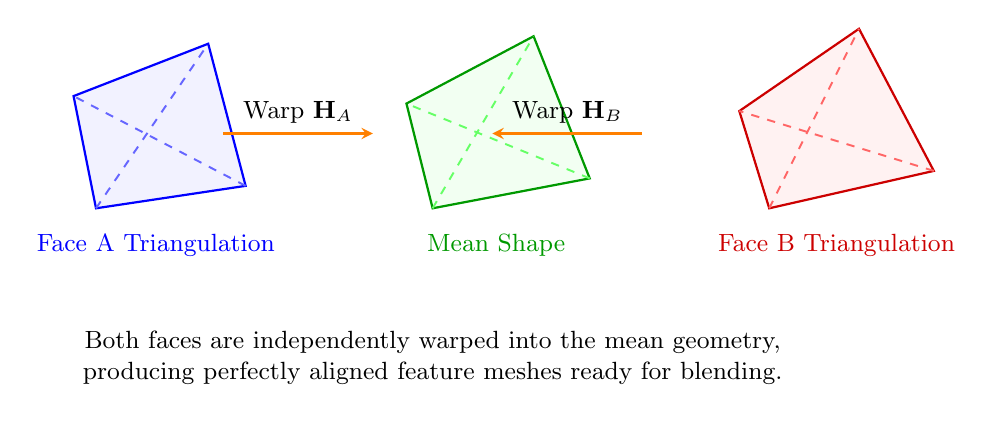
\begin{tikzpicture}[>=stealth, line width=0.7pt, scale=0.95]
    % Face A (Left)
    \begin{scope}[shift={(-4.5, 0)}]
        \coordinate (A1) at (0,0);
        \coordinate (A2) at (2,0.3);
        \coordinate (A3) at (1.5,2.2);
        \coordinate (A4) at (-0.3,1.5);
        \draw[thick, blue, fill=blue!5] (A1) -- (A2) -- (A3) -- (A4) -- cycle;
        \draw[dashed, blue!60] (A1) -- (A3);
        \draw[dashed, blue!60] (A2) -- (A4);
        \node[blue, font=\small] at (0.8, -0.5) {Face~A Triangulation};
    \end{scope}

    % Face B (Right)
    \begin{scope}[shift={(4.5, 0)}]
        \coordinate (B1) at (0,0);
        \coordinate (B2) at (2.2,0.5);
        \coordinate (B3) at (1.2,2.4);
        \coordinate (B4) at (-0.4,1.3);
        \draw[thick, red!80!black, fill=red!5] (B1) -- (B2) -- (B3) -- (B4) -- cycle;
        \draw[dashed, red!60] (B1) -- (B3);
        \draw[dashed, red!60] (B2) -- (B4);
        \node[red!80!black, font=\small] at (0.9, -0.5) {Face~B Triangulation};
    \end{scope}

    % Mean Shape (Center)
    \begin{scope}[shift={(0, 0)}]
        \coordinate (M1) at (0,0);
        \coordinate (M2) at (2.1,0.4);
        \coordinate (M3) at (1.35,2.3);
        \coordinate (M4) at (-0.35,1.4);
        \draw[thick, green!60!black, fill=green!5] (M1) -- (M2) -- (M3) -- (M4) -- cycle;
        \draw[dashed, green!60] (M1) -- (M3);
        \draw[dashed, green!60] (M2) -- (M4);
        \node[green!60!black, font=\small] at (0.85, -0.5) {Mean Shape};
    \end{scope}

    % Arrows
    \draw[->, thick, orange] (-2.8, 1.0) -- node[above, sloped, black, font=\small] {Warp $\mathbf{H}_A$} (-0.8, 1.0);
    \draw[<-, thick, orange] (0.8, 1.0) -- node[above, sloped, black, font=\small] {Warp $\mathbf{H}_B$} (2.8, 1.0);

    % Bottom caption
    \node[align=center, font=\small] at (0, -2.0) {Both faces are independently warped into the mean geometry,\\ producing perfectly aligned feature meshes ready for blending.};
\end{tikzpicture}
\caption{Complete warping concept. The Delaunay triangulation is computed once on the mean shape. The same connectivity is projected onto both input faces via index correspondence. Each face is then warped into the mean geometry using its own set of piecewise affine transforms, aligning all facial features without distortion discontinuities.}
\label{fig:complete-warp-concept}
\end{figure}

\subsection{Computing the Affine Warp for Each Triangle}

For a given triangle $T_A^{(p)} = (\mathbf{a}_i, \mathbf{a}_j, \mathbf{a}_k)$ and its target $T_{\text{mean}}^{(p)} = (\mathbf{m}_i, \mathbf{m}_j, \mathbf{m}_k)$, we seek an affine transform that maps every point inside the source triangle to the target triangle. In homogeneous coordinates, a 2D affine transform is represented by a $3 \times 3$ matrix:
\begin{equation}
    \begin{bmatrix} x' \\ y' \\ 1 \end{bmatrix}
    =
    \mathbf{H}
    \begin{bmatrix} x \\ y \\ 1 \end{bmatrix},
    \quad \text{where} \quad
    \mathbf{H} =
    \begin{bmatrix}
        h_{11} & h_{12} & t_x \\
        h_{21} & h_{22} & t_y \\
        0 & 0 & 1
    \end{bmatrix}.
\end{equation}
The top-left $2 \times 2$ block handles rotation, scaling, and shearing; the rightmost column handles translation.

Because three non-collinear points uniquely determine a 2D affine transform, we can solve for $\mathbf{H}_A$ by stacking the three vertex correspondences into a matrix equation:
\begin{equation}
    \underbrace{
    \begin{bmatrix}
        m_{ix} & m_{jx} & m_{kx} \\
        m_{iy} & m_{jy} & m_{ky} \\
        1 & 1 & 1
    \end{bmatrix}}_{\mathbf{X}_{\text{mean}}}
    =
    \mathbf{H}_A
    \underbrace{
    \begin{bmatrix}
        a_{ix} & a_{jx} & a_{kx} \\
        a_{iy} & a_{jy} & a_{ky} \\
        1 & 1 & 1
    \end{bmatrix}}_{\mathbf{X}_A}.
\end{equation}
Assuming the source triangle is non-degenerate (its vertices are not collinear), $\mathbf{X}_A$ is invertible. We solve for the forward warp matrix:
\begin{equation}
    \mathbf{H}_A = \mathbf{X}_{\text{mean}} \, \mathbf{X}_A^{-1}.
\end{equation}
The exact same procedure yields $\mathbf{H}_B = \mathbf{X}_{\text{mean}} \, \mathbf{X}_B^{-1}$ for Face~B. The explicit inverse of a $3 \times 3$ matrix can be computed via cofactors, Cramer's rule, or standard numerical routines. For the affine case, the bottom row of $\mathbf{H}_A$ is always $(0, 0, 1)$, so in practice we only need to invert the $2 \times 3$ augmented system or solve two independent $3 \times 3$ linear systems for the $x$ and $y$ components separately.

\subsection{Inverse Warping (Backward Mapping)}

A naive approach would apply the forward transform $\mathbf{H}_A$ to every pixel inside $T_A^{(p)}$ and write the color to the corresponding location in the output image. This \emph{forward mapping} has a critical flaw: the transformed coordinates will almost always fall between integer pixel locations, and multiple source pixels may map to the same destination or leave destination pixels completely unassigned. The result is a warped image with \emph{holes} and overlapping samples.

The standard solution is \emph{inverse warping} (also called backward mapping). Instead of asking ``where does this source pixel go?'', we ask ``which source pixel belongs to this destination pixel?''. The procedure is:

\begin{enumerate}
    \item Allocate a blank output image $W$ with the same dimensions as the mean shape canvas.
    \item Precompute the \emph{inverse} affine matrices $\mathbf{H}_A^{-1}$ and $\mathbf{H}_B^{-1}$ for every triangle. These map from the mean shape \emph{back} to the original face geometry.
    \item For each output pixel at integer coordinates $(x, y)$:
    \begin{enumerate}
        \item \textbf{Locate} which mean triangle $T_{\text{mean}}^{(p)}$ contains $(x, y)$.
        \item \textbf{Back-project} using the inverse matrix:
        \begin{equation}
            \begin{bmatrix} x_s \\ y_s \\ 1 \end{bmatrix}
            = \mathbf{H}_A^{-1}
            \begin{bmatrix} x \\ y \\ 1 \end{bmatrix}.
        \end{equation}
        This yields continuous (non-integer) source coordinates $(x_s, y_s)$.
        \item \textbf{Sample} the source image $I_A$ at $(x_s, y_s)$ using bilinear interpolation.
        \item \textbf{Write} the interpolated color value to $W(x, y)$.
    \end{enumerate}
\end{enumerate}

Because we visit every output pixel exactly once and fill it via back-projection, inverse warping \emph{guarantees} a complete, hole-free image.

\paragraph{Bilinear Interpolation.}
Since $(x_s, y_s)$ are real-valued coordinates, we sample the four nearest integer pixels and blend them according to their fractional distances. Let $x_0 = \lfloor x_s \rfloor$, $y_0 = \lfloor y_s \rfloor$, $u = x_s - x_0$, and $v = y_s - y_0$. The interpolated intensity is:
\begin{align}
    I(x_s, y_s) =\; &(1-u)(1-v)\, I(x_0, y_0) \;+\; u(1-v)\, I(x_0+1, y_0) \nonumber \\
                  &+\; (1-u)v\, I(x_0, y_0+1) \;+\; uv\, I(x_0+1, y_0+1).
\end{align}
This formula is applied independently to each color channel (R, G, B). Bilinear interpolation produces smooth gradients and avoids the blocky artifacts of nearest-neighbor sampling, while remaining computationally cheap.

\subsection{Point-in-Triangle Test Using Barycentric Coordinates}

Step 3(a) above requires an efficient way to determine which triangle ``owns'' a given output pixel. Barycentric coordinates, introduced in Section~3, serve this purpose elegantly.

For a target point $\mathbf{p} = (x, y)$ and a mean triangle with vertices $\mathbf{m}_i, \mathbf{m}_j, \mathbf{m}_k$, we compute the barycentric weights $(w_i, w_j, w_k)$ by solving:
\begin{equation}
    \mathbf{p} = w_i \mathbf{m}_i + w_j \mathbf{m}_j + w_k \mathbf{m}_k,
    \quad \text{subject to} \quad w_i + w_j + w_k = 1.
\end{equation}
This is a $2 \times 2$ linear system (after eliminating $w_k = 1 - w_i - w_j$) that can be solved analytically using cross-products or determinants. The membership test is then trivial:
\begin{equation}
    \mathbf{p} \in T_{\text{mean}}^{(p)} \quad \Longleftrightarrow \quad
    0 \leq w_i \leq 1 \;\land\; 0 \leq w_j \leq 1 \;\land\; 0 \leq w_k \leq 1.
\end{equation}
Since the weights sum to one, it is sufficient to check that all three are non-negative. If the condition holds, the point lies inside (or exactly on the edge of) the triangle. Additionally, these same weights can be reused for texture coordinate interpolation if needed, though for pure color warping we rely on the inverse matrix.

\subsection{Bounding Box Optimization}

Testing every output pixel against every triangle would result in $\mathcal{O}(N_{\text{pixels}} \times N_{\text{triangles}})$ complexity, which is prohibitively slow for high-resolution images. We can dramatically accelerate this using a \emph{bounding box} culling strategy:

\begin{enumerate}
    \item For each mean triangle $T_{\text{mean}}^{(p)}$, compute its axis-aligned bounding box (AABB):
    \[
        x_{\min} = \lfloor \min(m_{ix}, m_{jx}, m_{kx}) \rfloor, \quad
        x_{\max} = \lceil \max(m_{ix}, m_{jx}, m_{kx}) \rceil,
    \]
    and similarly for $y_{\min}, y_{\max}$.
    \item Iterate \emph{only} over integer pixels $(x, y)$ satisfying $x_{\min} \leq x \leq x_{\max}$ and $y_{\min} \leq y \leq y_{\max}$.
    \item Perform the barycentric point-in-triangle test only for pixels inside the bounding box.
\end{enumerate}

Since a triangle's bounding box typically contains only a small constant factor more pixels than the triangle itself, this reduces the effective complexity to nearly $\mathcal{O}(N_{\text{pixels}})$ overall: each output pixel is tested against only the few triangles whose bounding boxes overlap it, and exactly one test succeeds. This optimization is standard in all GPU and software rasterizers.

\subsection{Handling the Background}

The Delaunay triangulation covers exactly the \emph{convex hull} of the landmark set. Everything outside this hull---hair, ears, neck, shoulders, and background---falls outside all triangles and will remain unfilled after the warping step. Several strategies exist to handle these regions:

\begin{description}
    \item[Direct Passthrough (Copy Original):] For pixels outside the convex hull, simply copy the original unwarped pixel from Face~A (or Face~B). This is the simplest approach and works well when the background is uniform or when the hull tightly covers the face. The transition at the hull boundary may show a slight geometric discontinuity if the face edge aligns poorly with the outermost landmarks.

    \item[Extended Triangulation with Border Points:] Add four artificial ``corner'' landmarks at the image boundaries (e.g., $(0,0), (W,0), (W,H), (0,H)$) and optionally midway points along each edge. Recompute the Delaunay triangulation including these points. The triangles connecting the convex hull to the image border form a smooth extension field that gently warps the background towards the mean shape, eliminating hard cutoff lines.

    \item[Masking and Alpha Compositing:] Render the warped face into a separate layer with an alpha mask derived from the convex hull. Composite this layer over an unwarped background layer using standard alpha blending:
    \[
        C_{\text{final}} = \alpha \, C_{\text{warped}} + (1 - \alpha) \, C_{\text{background}},
    \]
    where $\alpha = 1$ inside the hull and smoothly feathers to $0$ near the boundary. This gives the most control over edge appearance and is the standard approach in professional morphing software.
\end{description}

In practice, a hybrid approach works best: extend the triangulation with border points to cover the entire image, then apply the piecewise warp uniformly. Triangles far from the face landmarks undergo nearly identity transforms, preserving the background naturally while ensuring complete pixel coverage.

\subsection{Complete Warping Procedure}

Algorithm~\ref{alg:piecewise-warp} summarizes the full piecewise affine warping pipeline for a single input face. Running it twice (once for Face~A, once for Face~B) produces two geometrically aligned images ready for cross-dissolve blending.

\begin{figure}[h]
\centering
\fbox{\begin{minipage}{0.9\textwidth}
\textbf{Algorithm:} Piecewise Affine Inverse Warp\\[4pt]
\textbf{Input:} Source image $I$, landmarks $L_{\text{src}} = \{\mathbf{a}_1, \dots, \mathbf{a}_n\}$, mean landmarks $M = \{\mathbf{m}_1, \dots, \mathbf{m}_n\}$, triangulation $\mathcal{T}$\\
\textbf{Output:} Warped image $W$ in mean shape geometry
\begin{enumerate}
    \item Initialize $W$ as a blank image with the canvas dimensions.
    \item \textbf{For each} triangle index $p = 1$ to $K$ in $\mathcal{T}$:
    \begin{enumerate}
        \item Retrieve vertex indices $(i, j, k)$ for triangle $p$.
        \item Construct $\mathbf{X}_{\text{src}}$ from $\mathbf{a}_i, \mathbf{a}_j, \mathbf{a}_k$ and $\mathbf{X}_{\text{mean}}$ from $\mathbf{m}_i, \mathbf{m}_j, \mathbf{m}_k$.
        \item Compute forward matrix: $\mathbf{H}^{(p)} = \mathbf{X}_{\text{mean}} \, \mathbf{X}_{\text{src}}^{-1}$.
        \item Compute inverse matrix: $\mathbf{H}_{\text{inv}}^{(p)} = \left(\mathbf{H}^{(p)}\right)^{-1}$.
        \item Compute bounding box $(x_{\min}, x_{\max}, y_{\min}, y_{\max})$ of $T_{\text{mean}}^{(p)}$.
    \end{enumerate}
    \item \textbf{For each} triangle $p = 1$ to $K$:
    \begin{enumerate}
        \item \textbf{For} $y$ from $y_{\min}$ to $y_{\max}$:
        \item \quad \textbf{For} $x$ from $x_{\min}$ to $x_{\max}$:
        \begin{enumerate}
            \item Compute barycentric weights $(w_i, w_j, w_k)$ of $(x, y)$ relative to $T_{\text{mean}}^{(p)}$.
            \item \textbf{If} $w_i \geq 0$ and $w_j \geq 0$ and $w_k \geq 0$:
            \begin{enumerate}
                \item Back-project: $\begin{bmatrix} x_s \\ y_s \\ 1 \end{bmatrix} = \mathbf{H}_{\text{inv}}^{(p)} \begin{bmatrix} x \\ y \\ 1 \end{bmatrix}$.
                \item Sample source: $C = \text{BilinearInterp}(I, x_s, y_s)$.
                \item Write output: $W(x, y) \gets C$.
            \end{enumerate}
        \end{enumerate}
    \end{enumerate}
    \item \textbf{Return} $W$.
\end{enumerate}
\end{minipage}}
\caption{Complete piecewise affine inverse warping algorithm. The affine matrices and bounding boxes are precomputed once per triangle (Step 2), then the rasterization loop (Step 3) fills the output image efficiently.}
\label{alg:piecewise-warp}
\end{figure}

The computational cost is dominated by Step 3, which touches every pixel in the convex hull exactly once. With $K$ triangles and image resolution $H \times W$, the complexity is $\mathcal{O}(HW + K)$, where the linear term comes from matrix precomputation and the dominant $HW$ term comes from pixel-level sampling. In typical face morphing, $K \approx 100\text{--}200$ triangles and $HW \approx 10^6$ pixels, making the per-frame warp easily real-time on modern hardware.
\section{Image Blending}

After piecewise affine warping, both Face~A and Face~B have been rendered into the same geometric
space --- the mean shape. Their features are now spatially aligned: the left eye of Face~A sits at
the same pixel coordinates as the left eye of Face~B, and so on for every landmark and every point
inside every Delaunay triangle. The geometry is resolved. What remains is to combine the
\emph{appearance} of the two warped images into a single result.

This section explains how to blend the warped images, how to generate an entire morph animation,
why the order of operations matters, and what advanced techniques exist beyond simple alpha
blending.

\subsection{The Blending Problem}

Consider the state of the pipeline at this point. We have:

\begin{itemize}
    \item $W_A(x, y)$ --- the image of Face~A warped from its original shape to the mean shape.
    \item $W_B(x, y)$ --- the image of Face~B warped from its original shape to the mean shape.
    \item Both images share the same canvas dimensions, the same pixel grid, and the same
          landmark geometry.
\end{itemize}

The challenge is to produce a single image $O(x, y)$ that combines information from both
$W_A$ and $W_B$ in a way that is visually natural. We want:

\begin{enumerate}
    \item \textbf{Detail preservation.} Both faces contribute information. The output should
          retain recognizable features from each input.
    \item \textbf{No visible seams.} The transition between contributions from the two faces
          should be invisible --- no hard edges, no sudden color jumps.
    \item \textbf{Controllable balance.} We should be able to adjust how much each face
          contributes, ranging from pure Face~A through a 50/50 average to pure Face~B.
\end{enumerate}

The simplest solution that satisfies all three requirements is \textbf{linear alpha blending},
also known as a cross-dissolve. More sophisticated techniques exist for eliminating subtle
artifacts, which we cover later in this section.

\subsection{Simple Alpha Blending (Cross-Dissolve)}

The most common and intuitive approach to image blending is a weighted linear combination.
For each pixel $(x, y)$ in the output image:

\begin{equation}
    \label{eq:alpha-blend-scalar}
    O(x, y) = \alpha \cdot W_A(x, y) + (1 - \alpha) \cdot W_B(x, y),
\end{equation}

where $\alpha \in [0, 1]$ is the blending parameter that controls the relative contribution of
each face, and $O(x, y)$ is the resulting pixel value.

\paragraph{Vector form for RGB.} Images have three color channels. Let us write each pixel as
a column vector in $\mathbb{R}^3$:

\begin{equation}
    \mathbf{w}_A(x, y) = \begin{bmatrix}
        W_{A,R}(x, y) \\
        W_{A,G}(x, y) \\
        W_{A,B}(x, y)
    \end{bmatrix},
    \qquad
    \mathbf{w}_B(x, y) = \begin{bmatrix}
        W_{B,R}(x, y) \\
        W_{B,G}(x, y) \\
        W_{B,B}(x, y)
    \end{bmatrix}.
\end{equation}

The blended output vector is then:

\begin{equation}
    \label{eq:alpha-blend-vector}
    \mathbf{o}(x, y) = \alpha \cdot \mathbf{w}_A(x, y) + (1 - \alpha) \cdot \mathbf{w}_B(x, y).
\end{equation}

Written component-wise, this expands to three independent equations --- one per channel:

\begin{align}
    O_R(x, y) &= \alpha \cdot W_{A,R}(x, y) + (1 - \alpha) \cdot W_{B,R}(x, y), \\
    O_G(x, y) &= \alpha \cdot W_{A,G}(x, y) + (1 - \alpha) \cdot W_{B,G}(x, y), \\
    O_B(x, y) &= \alpha \cdot W_{A,B}(x, y) + (1 - \alpha) \cdot W_{B,B}(x, y).
\end{align}

\paragraph{Geometric interpretation.} For a fixed pixel location $(x, y)$, the two input color
vectors $\mathbf{w}_A(x, y)$ and $\mathbf{w}_B(x, y)$ define the endpoints of a line segment in
$\mathbb{R}^3$ color space. Equation~\eqref{eq:alpha-blend-vector} places the output
$\mathbf{o}(x, y)$ somewhere on that segment. As $\alpha$ varies from 0 to 1, the output traces
the entire segment --- a straight-line path between the two colors.

\paragraph{Special values of $\alpha$.}

\begin{itemize}
    \item $\alpha = 1.0$ --- the output is entirely Face~A in the mean shape.
          $O = W_A$.
    \item $\alpha = 0.5$ --- equal contribution from both faces. This is the
          \textbf{face average}:
          \begin{equation}
              O(x, y) = \tfrac{1}{2}\, W_A(x, y) + \tfrac{1}{2}\, W_B(x, y).
          \end{equation}
    \item $\alpha = 0.0$ --- the output is entirely Face~B in the mean shape.
          $O = W_B$.
\end{itemize}

Any value between 0 and 1 produces a valid blend. The parameter $\alpha$ gives us continuous
control over the appearance balance.

\subsection{The Morph Sequence: Creating a Transition Animation}

One of the most visually striking applications of face morphing is creating a smooth transition
animation from Face~A to Face~B. Rather than computing a single blend at $\alpha = 0.5$, we
generate a sequence of frames where $\alpha$ sweeps continuously from 0 to 1.

\subsubsection{Frame Generation}

To produce an animation with $N$ frames, we sample $\alpha$ at $N$ uniformly spaced values:

\begin{equation}
    \alpha_k = \frac{k}{N - 1}, \qquad k = 0, 1, 2, \ldots, N - 1.
\end{equation}

For example, with $N = 30$ frames:

\begin{equation}
    \alpha = 0,\; \tfrac{1}{29},\; \tfrac{2}{29},\; \ldots,\; \tfrac{28}{29},\; 1.
\end{equation}

For each frame $k$, both the \emph{geometry} and the \emph{colors} change simultaneously.
Using a normalized time parameter $t = \alpha_k \in [0, 1]$:

\begin{itemize}
    \item \textbf{Geometry interpolation.} The landmarks for the mean shape at time $t$ are:
          \begin{equation}
              \label{eq:landmark-interp}
              \mathbf{m}_i(t) = (1 - t)\, \mathbf{a}_i + t\, \mathbf{b}_i,
              \qquad i = 1, \ldots, N_{\text{landmarks}},
          \end{equation}
          where $\mathbf{a}_i$ and $\mathbf{b}_i$ are the landmark positions in Face~A and
          Face~B respectively.
    \item \textbf{Color interpolation.} The blended pixel values at time $t$ are:
          \begin{equation}
              \label{eq:color-interp}
              I(x, y; t) = (1 - t) \cdot I_{A,\text{warped}}(x, y)
                         + t \cdot I_{B,\text{warped}}(x, y).
          \end{equation}
\end{itemize}

Together, Equations~\eqref{eq:landmark-interp} and~\eqref{eq:color-interp} define a continuous
family of images parameterized by $t$. Sampling this family at discrete time steps produces the
frames of the morph animation.

\subsubsection{Frame Rate and Frame Count}

The choice of $N$ and the display frame rate determines the duration and smoothness of the
animation:

\begin{itemize}
    \item For a \textbf{2-second morph} at 30~fps, we need $N = 60$ frames with
          $\alpha_k = k / 59$.
    \item For a \textbf{3-second morph} at 24~fps (cinematic), we need $N = 72$ frames.
    \item For a quick preview, $N = 30$ frames at 15~fps gives a 2-second animation that
          is smooth enough to evaluate.
\end{itemize}

In general, the perceived smoothness improves with more frames, but the improvement follows
diminishing returns. Beyond about 60 frames for a 2--3 second morph, additional frames are no
longer perceptible to the human eye.

\subsubsection{Implementation}

A practical Python implementation:

\begin{minted}{python}
import numpy as np
from PIL import Image

N = 60  # number of frames (e.g., 60 frames at 30 fps = 2 seconds)
alphas = np.linspace(0.0, 1.0, N)

frames = []
for alpha in alphas:
    # Geometry: interpolate landmarks for this frame
    landmarks_t = (1 - alpha) * landmarks_A + alpha * landmarks_B

    # Warp both faces to the intermediate geometry
    warped_A = piecewise_affine_warp(img_A, landmarks_A, landmarks_t, triangles)
    warped_B = piecewise_affine_warp(img_B, landmarks_B, landmarks_t, triangles)

    # Blend colors
    frame = (1 - alpha) * warped_A.astype(np.float64) + \
             alpha  * warped_B.astype(np.float64)
    frame = np.clip(frame, 0, 255).astype(np.uint8)
    frames.append(Image.fromarray(frame))

# Save as animated GIF
frames[0].save('morph_sequence.gif',
               save_all=True,
               append_images=frames[1:],
               duration=67,  # ms per frame (~15 fps)
               loop=0)
\end{minted}

\begin{figure}[htbp]
\centering
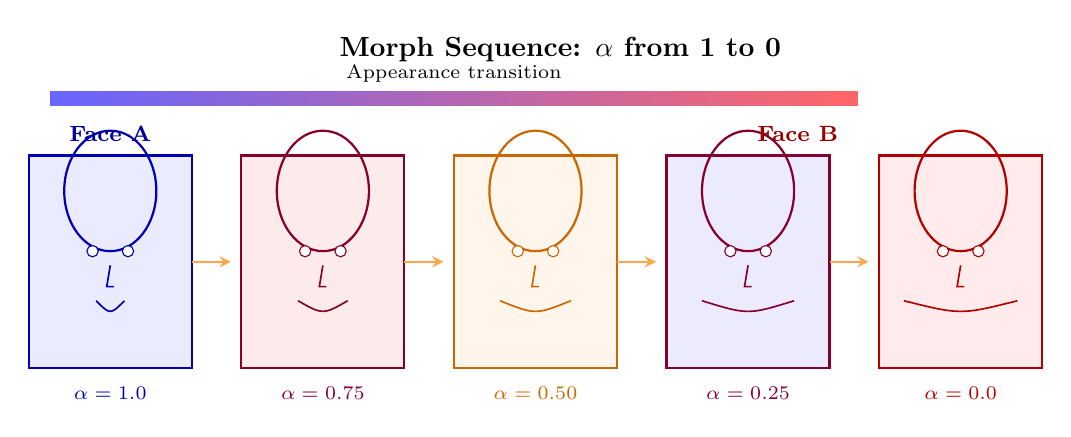
\begin{tikzpicture}[>=stealth, scale=0.9]
    % Title
    \node[font=\normalsize\bfseries] at (7.5, 5.0) {Morph Sequence: $\alpha$ from 1 to 0};

    % Five panels
    \foreach \i/\lbl/\bg/\fg in {%
        0/{$\alpha = 1.0$}/blue!8/blue!70!black,%
        1/{$\alpha = 0.75$}/blue!8!red!8/purple!70!black,%
        2/{$\alpha = 0.50$}/orange!8/orange!80!black,%
        3/{$\alpha = 0.25$}/red!8!blue!8/purple!70!black,%
        4/{$\alpha = 0.0$}/red!8/red!70!black%
    } {
        \pgfmathsetmacro{\xpos}{\i * 3.0}

        % Panel border
        \filldraw[thick, draw=\fg, fill=\bg] (\xpos, 0.5) rectangle (\xpos + 2.3, 3.5);

        % Stylized face outline inside panel
        \begin{scope}[shift={(\xpos + 1.15, 2.0)}]
            % Head shape
            \draw[color=\fg, line width=0.8pt] (0, 1.0) ellipse [x radius=0.65, y radius=0.85];
            % Eyes
            \filldraw[color=\fg, fill=white] (-0.25, 0.15) circle (0.08);
            \filldraw[color=\fg, fill=white] (0.25, 0.15) circle (0.08);
            % Nose
            \draw[color=\fg, line width=0.6pt] (0, -0.05) -- (-0.05, -0.35) -- (0.05, -0.35);
            % Mouth - varies with alpha
            \pgfmathsetmacro{\mouthwidth}{0.2 + 0.15*\i}
            \draw[color=\fg, line width=0.6pt] (-\mouthwidth, -0.55) .. controls (0, -0.75) .. (\mouthwidth, -0.55);
        \end{scope}

        % Alpha label below
        \node[font=\scriptsize, color=\fg] at (\xpos + 1.15, 0.15) {\lbl};

        % Arrows between panels
        \ifnum \i < 4
            \draw[->, thick, orange!70] (\xpos + 2.3, 2.0) -- (\xpos + 2.85, 2.0);
        \fi
    }

    % Gradient bar at top
    \shade[left color=blue!60, right color=red!60] (0.3, 4.2) rectangle (11.7, 4.4);
    \node[font=\scriptsize] at (6.0, 4.65) {Appearance transition};

    % Face labels
    \node[font=\footnotesize\bfseries, blue!60!black] at (1.15, 3.8) {Face~A};
    \node[font=\footnotesize\bfseries, red!60!black] at (10.85, 3.8) {Face~B};
\end{tikzpicture}
\caption{The morph sequence: five key frames showing a smooth transition from Face~A
($\alpha = 1.0$) through intermediate blends to Face~B ($\alpha = 0.0$). The geometry (mean
shape) evolves at each frame via landmark interpolation, and the colors blend via alpha
compositing. The gradient bar illustrates the continuous appearance transition. Connecting
arrows indicate the temporal progression.}
\label{fig:morph-sequence}
\end{figure}

\subsection{Why We Blend in Mean Shape Space}

The order of operations in the face morphing pipeline is not arbitrary. The correct sequence is:

\begin{center}
\fbox{Warp both faces to mean shape} $\;\longrightarrow\;$ \fbox{Blend the warped images}
\end{center}

It is instructive to understand why the reverse order fails.

\subsubsection{The Wrong Order: Blend Then Warp}

Suppose we first blend the \emph{original} (unwarped) Face~A and Face~B, and then attempt to
warp the result to the mean shape:

\begin{center}
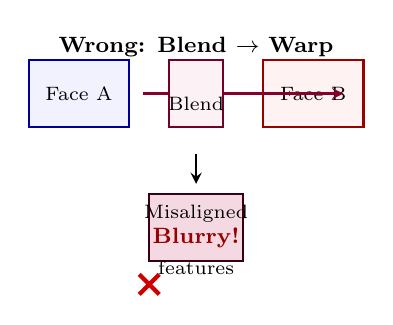
\begin{tikzpicture}[>=stealth, scale=0.85]
    % Top row: wrong order
    \node[font=\bfseries\footnotesize] at (0, 3.2) {Wrong: Blend $\rightarrow$ Warp};

    % Original faces
    \filldraw[thick, draw=blue!60!black, fill=blue!5] (-2.5, 2.0) rectangle (-1.0, 3.0);
    \node[font=\scriptsize, align=center] at (-1.75, 2.5) {Face~A};

    \filldraw[thick, draw=red!60!black, fill=red!5] (1.0, 2.0) rectangle (2.5, 3.0);
    \node[font=\scriptsize, align=center] at (1.75, 2.5) {Face~B};

    % Blend arrow
    \draw[->, thick, purple!70!black] (-0.8, 2.5) -- (-0.1, 2.5);
    \draw[<-, thick, purple!70!black] (0.1, 2.5) -- (0.8, 2.5);

    % Blended (unwarped)
    \filldraw[thick, draw=purple!60!black, fill=purple!5] (-0.4, 2.0) rectangle (0.4, 3.0);
    \node[font=\scriptsize, align=center] at (0, 2.35) {Blend};

    % Warp arrow
    \draw[->, thick, purple!70!black] (0.4, 2.5) -- (2.2, 2.5);
    \draw[->, thick] (0, 1.6) -- (0, 1.15);

    % Result (warped blend)
    \filldraw[thick, draw=purple!30!black, fill=purple!15] (-0.7, 0.0) rectangle (0.7, 1.0);
    \node[font=\footnotesize\bfseries, red!60!black] at (0, 0.35) {Blurry!};
    \node[font=\scriptsize, align=center] at (0, 0.7) {Misaligned};
    \node[font=\scriptsize, align=center] at (0, -0.1) {features};

    % X mark
    \draw[red!80!black, line width=1.5pt] (-0.85, -0.5) -- (-0.55, -0.2);
    \draw[red!80!black, line width=1.5pt] (-0.55, -0.5) -- (-0.85, -0.2);
\end{tikzpicture}
\end{center}

The problem is geometric: Face~A's left eye might be at pixel $(120, 80)$ while Face~B's left
eye is at $(150, 90)$. If we blend first, the resulting pixel at $(120, 80)$ is a mix of
Face~A's eye and Face~B's \emph{cheek} (since Face~B's eye is elsewhere). The blend already
contains a ghosted, misaligned superposition. Warping this blurred result to the mean shape
cannot recover the lost detail --- it merely deforms the blur.

More formally, the pixel-wise blending in Equation~\eqref{eq:alpha-blend-scalar} assumes that
$W_A(x, y)$ and $W_B(x, y)$ represent \emph{corresponding} image content at position $(x, y)$.
When the images are not geometrically aligned, this assumption is violated, and the linear
combination no longer has a meaningful interpretation.

\subsubsection{The Correct Order: Warp Then Blend}

Now consider the correct sequence. First, each face is warped independently to the mean shape:

\begin{center}
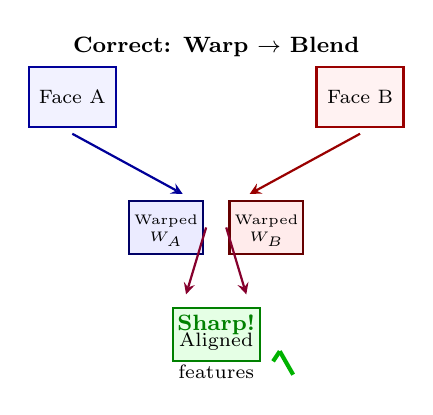
\begin{tikzpicture}[>=stealth, scale=0.85]
    % Bottom row: correct order
    \node[font=\bfseries\footnotesize] at (0, 3.2) {Correct: Warp $\rightarrow$ Blend};

    % Original faces
    \filldraw[thick, draw=blue!60!black, fill=blue!5] (-2.8, 2.0) rectangle (-1.5, 2.9);
    \node[font=\scriptsize, align=center] at (-2.15, 2.45) {Face~A};

    \filldraw[thick, draw=red!60!black, fill=red!5] (1.5, 2.0) rectangle (2.8, 2.9);
    \node[font=\scriptsize, align=center] at (2.15, 2.45) {Face~B};

    % Warp arrows (down and inward)
    \draw[->, thick, blue!60!black] (-2.15, 1.9) -- (-0.5, 1.0);
    \draw[->, thick, red!60!black] (2.15, 1.9) -- (0.5, 1.0);

    % Warped faces in mean shape
    \filldraw[thick, draw=blue!40!black, fill=blue!8] (-1.3, 0.1) rectangle (-0.2, 0.9);
    \node[font=\tiny, align=center] at (-0.75, 0.45) {Warped\\$W_A$};

    \filldraw[thick, draw=red!40!black, fill=red!8] (0.2, 0.1) rectangle (1.3, 0.9);
    \node[font=\tiny, align=center] at (0.75, 0.45) {Warped\\$W_B$};

    % Blend arrows
    \draw[->, thick, purple!70!black] (-0.15, 0.5) -- (-0.45, -0.5);
    \draw[->, thick, purple!70!black] (0.15, 0.5) -- (0.45, -0.5);

    % Blended result
    \filldraw[thick, draw=green!50!black, fill=green!10] (-0.65, -1.5) rectangle (0.65, -0.7);
    \node[font=\footnotesize\bfseries, green!50!black] at (0, -0.95) {Sharp!};
    \node[font=\scriptsize, align=center] at (0, -1.2) {Aligned};
    \node[font=\scriptsize, align=center] at (0, -1.65) {features};

    % Checkmark
    \draw[green!70!black, line width=1.5pt] (0.85, -1.5) -- (0.95, -1.35);
    \draw[green!70!black, line width=1.5pt] (0.95, -1.35) -- (1.15, -1.7);
\end{tikzpicture}
\end{center}

After warping, both $W_A$ and $W_B$ have Face~A's left eye and Face~B's left eye at the
\emph{same} pixel coordinate in the mean-shape canvas. The blending operation now combines
corresponding features with corresponding features. The result is sharp because the input
to the blend is already geometrically registered.

The key insight is that the Delaunay triangulation and piecewise affine warp establish a
``pixel correspondence'' between the two images. Once this correspondence is established,
simple linear blending is sufficient to produce a natural-looking composite.

\subsubsection{Summary of Artifact Comparison}

\begin{table}[htbp]
\centering
\caption{Comparison of blending orders and their visual consequences.}
\label{tab:blend-order}
\begin{tabular}{@{}lcc@{}}
\toprule
& \textbf{Blend $\rightarrow$ Warp} & \textbf{Warp $\rightarrow$ Blend} \\
\midrule
Spatial alignment & No (features at different locations) & Yes (both in mean shape) \\
Feature correspondence & Pixel $p$ in A $\neq$ pixel $p$ in B & Pixel $p$ in A $\approx$ pixel $p$ in B \\
Blending artifacts & Ghosting, blur, doubling & None (assuming good landmarks) \\
Geometric distortion & Warped blur (irreversible) & None \\
Final quality & Poor & Excellent \\
\bottomrule
\end{tabular}
\end{table}

\subsection{Advanced Blending Techniques}

While simple alpha blending produces good results for most face morphing applications, several
advanced techniques can further improve quality in challenging cases.

\subsubsection{Multi-Band (Laplacian Pyramid) Blending}

Multi-band blending decomposes images into frequency bands using a \textbf{Laplacian pyramid}
and blends each band with a different strategy. The intuition is:

\begin{itemize}
    \item \textbf{Low frequencies} (smooth gradients, overall brightness) can be blended with a
          gentle, gradual transition. These carry the overall color and lighting.
    \item \textbf{High frequencies} (edges, fine texture) benefit from a sharper transition to
          avoid blurring or visible seams along triangle boundaries.
\end{itemize}

\paragraph{Pyramid decomposition.} The Laplacian pyramid is constructed as follows:

\begin{enumerate}
    \item Start with the image $I_0 = I$ at full resolution.
    \item \textbf{Gaussian pyramid:} Repeatedly blur and downsample:
          \begin{equation}
              I_{k} = \text{blur}\bigl(\text{downsample}(I_{k-1})\bigr), \qquad k = 1, 2, \ldots, L,
          \end{equation}
          where $L$ is the pyramid depth.
    \item \textbf{Laplacian pyramid:} At each level, compute the difference between the current
          level and the upsampled, blurred version of the next level:
          \begin{equation}
              \mathcal{L}_k = I_k - \text{upsample}\bigl(\text{blur}(I_{k+1})\bigr),
              \qquad k = 0, 1, \ldots, L - 1.
          \end{equation}
          The top level $\mathcal{L}_L = I_L$ is the coarsest Gaussian level.
\end{enumerate}

Each level $\mathcal{L}_k$ captures detail at a specific spatial frequency. The original image
can be perfectly reconstructed by summing all levels:

\begin{equation}
    I = \sum_{k=0}^{L} \mathcal{L}_k.
\end{equation}

For blending, we construct Laplacian pyramids for both $W_A$ and $W_B$, then blend each level
with its own weighting $\alpha_k$. Typically, $\alpha_k$ is more aggressive (closer to a
step function) at high frequencies and more gentle at low frequencies. The final blended image
is reconstructed by collapsing the blended pyramid.

This approach eliminates visible seams that can appear at triangle boundaries, because the
sharp discontinuities are pushed into the highest frequency bands where they are less
perceptible.

\subsubsection{Poisson Blending}

Poisson blending formulates the blending problem as solving a \textbf{Poisson equation} in the
gradient domain. Instead of directly averaging pixel values, it seeks an output image $O$ whose
gradient field best matches a target gradient, subject to boundary conditions:

\begin{equation}
    \Delta O = \nabla \cdot \mathbf{v},
\end{equation}

where $\mathbf{v}$ is the \emph{guidance vector field} (typically the gradient of one of the
input images or a combination), $\Delta$ is the Laplacian operator, and $\nabla \cdot$ is the
divergence.

In the context of face morphing, Poisson blending can be used to seamlessly merge the two
warped images by matching the gradients along triangle boundaries. It is more commonly used
for image compositing (pasting objects into new backgrounds) but can reduce seam artifacts in
morphing when the two faces have significantly different lighting or contrast.

The main drawback is computational cost: solving the Poisson equation requires solving a large
sparse linear system, typically via iterative methods (e.g., multigrid or conjugate gradient).

\subsubsection{Feature-Weighted Blending}

Instead of using a uniform $\alpha$ across the entire image, we can define a
\textbf{spatially-varying blending weight} $\alpha(x, y)$:

\begin{equation}
    O(x, y) = \alpha(x, y) \cdot W_A(x, y) + (1 - \alpha(x, y)) \cdot W_B(x, y).
\end{equation}

The weight function $\alpha(x, y)$ can be designed to emphasize facial regions where identity
is most recognizable:

\begin{itemize}
    \item \textbf{Eyes, nose, mouth:} Give higher weight to the face whose features are clearer
          or more expressive in these regions.
    \item \textbf{Face boundary / hairline:} Transition smoothly to avoid a visible seam where
          the face meets the background.
    \item \textbf{Smoothness:} The weight function itself must be smooth to avoid introducing
          new artifacts. A common choice is a Gaussian-weighted mask centered on each facial
          feature.
\end{itemize}

This technique gives the user fine-grained artistic control, allowing them to, for example,
preserve Face~A's eyes and smile while taking Face~B's jawline and forehead.

\subsubsection{Comparison of Techniques}

\begin{table}[htbp]
\centering
\caption{Comparison of blending techniques.}
\label{tab:blending-comparison}
\begin{tabular}{@{}lcccc@{}}
\toprule
\textbf{Technique} & \textbf{Complexity} & \textbf{Quality} & \textbf{Speed} & \textbf{When to Use} \\
\midrule
Alpha blending & Low & Good & Very fast & Default choice; most cases \\
Multi-band blending & Medium & Very good & Fast & Visible seams; lighting mismatch \\
Poisson blending & High & Excellent & Slow & Significant lighting/contrast differences \\
Feature-weighted & Medium & User-dependent & Fast & Artistic control; selective features \\
\bottomrule
\end{tabular}
\end{table}

For the vast majority of face morphing tasks, simple alpha blending with good landmark
correspondence produces excellent results. The advanced techniques are most valuable when
the input faces differ substantially in lighting, exposure, or background.

\subsection{Post-Processing}

After the blending step, a few optional post-processing operations can polish the final result.

\subsubsection{Color Correction}

If Face~A and Face~B have different overall brightness or color balance, the blended result may
appear slightly off. A simple correction matches the mean and variance of the output to the
inputs:

\begin{equation}
    O_{\text{corrected}}(x, y) = \sigma_{\text{target}}
        \cdot \frac{O(x, y) - \mu_O}{\sigma_O} + \mu_{\text{target}},
\end{equation}

where $\mu_O$ and $\sigma_O$ are the mean and standard deviation of the blended image, and
$\mu_{\text{target}}$, $\sigma_{\text{target}}$ are the desired statistics (e.g., the average
of the two input means). This is a per-channel operation applied independently to R, G, and B.

A simpler approach is to adjust the overall brightness so that the mean intensity of the output
equals the average of the mean intensities of the two warped inputs.

\subsubsection{Boundary Smoothing}

Minor artifacts can persist at Delaunay triangle edges after blending. A mild Gaussian blur
applied to the final result can help:

\begin{equation}
    O_{\text{smooth}}(x, y) = \sum_{u, v} G_\sigma(u, v) \cdot O(x - u, y - v),
\end{equation}

where $G_\sigma$ is a 2D Gaussian kernel with a small standard deviation
($\sigma \approx 0.5$--1.0 pixels). This is subtle enough to avoid noticeable loss of sharpness
while eliminating sub-pixel seams.

In practice:

\begin{minted}{python}
import cv2

# sigma = 0.8 is a gentle default
smoothed = cv2.GaussianBlur(blended, ksize=(3, 3), sigmaX=0.8)
\end{minted}

\subsubsection{Vignetting and Aesthetic Touches}

For presentation-quality output, post-processing may include:

\begin{itemize}
    \item \textbf{Vignetting:} Darken the image edges with a radially symmetric falloff to draw
          attention to the face center. Applied as a per-pixel multiplication:
          \begin{equation}
              O_{\text{vignette}}(x, y) = v(r) \cdot O(x, y), \quad
              r = \frac{\sqrt{(x - c_x)^2 + (y - c_y)^2}}{r_{\text{max}}},
          \end{equation}
          where $v(r)$ decreases from 1 at the center to about 0.7 at the corners.
    \item \textbf{Contrast enhancement:} A slight S-curve in the tone curve can make the result
          pop.
    \item \textbf{Cropping:} Tight crop to the face region removes any black borders or
          background artifacts from the warping step.
\end{itemize}

These steps are optional and depend on the intended use case. For algorithmic evaluation, raw
output without post-processing is preferred. For presentations, a light touch of vignetting
and contrast enhancement goes a long way.

\section{Complete Pipeline and Implementation}

By now we have covered every component of the feature-based face morphing algorithm. In this chapter we bring everything together: a complete worked-out pseudocode specification, a full Python implementation supporting both \texttt{dlib} and \texttt{MediaPipe} backends for landmark detection, a complexity analysis, and practical debugging tips.

\subsection{Full Algorithm Specification}

Algorithm~\ref{alg:face-morph} presents the complete face morphing procedure. The algorithm takes two input images $I_A$ and $I_B$, a choice of blending parameter $\alpha \in [0,1]$, and produces the morphed output image $O$.

\begin{algorithm}[t]
\caption{Feature-Based Face Morphing}
\label{alg:face-morph}
\begin{algorithmic}[1]
\Require Two face images $I_A, I_B$; blending weight $\alpha \in [0,1]$
\Ensure Morphed image $O$

\State $L_A \gets \texttt{detectLandmarks}(I_A)$ \Comment{68-point landmarks}
\State $L_B \gets \texttt{detectLandmarks}(I_B)$
\State $M \gets \{(a_i + b_i)/2 \mid (a_i, b_i) \in (L_A, L_B)\}$ \Comment{Mean shape}
\State $\texttt{triangles} \gets \texttt{delaunayTriangulate}(M)$
\State $O \gets \texttt{zeros like } I_A$
\ForAll{triangle $(i, j, k)$ in \texttt{triangles}}
    \State $T_M \gets (M_i, M_j, M_k)$ \Comment{Triangle in mean shape}
    \State $T_A \gets (L_{A,i}, L_{A,j}, L_{A,k})$
    \State $T_B \gets (L_{B,i}, L_{B,j}, L_{B,k})$
    \State $H_A \gets \texttt{computeAffineTransform}(T_A, T_M)$
    \State $H_B \gets \texttt{computeAffineTransform}(T_B, T_M)$
    \State Compute $H_A^{-1}, H_B^{-1}$ \Comment{Inverse warp matrices}
    \State $[\texttt{xmin}, \texttt{xmax}, \texttt{ymin}, \texttt{ymax}] \gets \texttt{boundingBox}(T_M)$
    \For{$y$ from $\texttt{ymin}$ to $\texttt{ymax}$}
        \For{$x$ from $\texttt{xmin}$ to $\texttt{xmax}$}
            \State \textcolor{gray}{\texttt{// Inverse map to source coordinates}}
            \State $(x_A, y_A) \gets H_A^{-1} \cdot (x, y, 1)$
            \State $(x_B, y_B) \gets H_B^{-1} \cdot (x, y, 1)$
            \State \textcolor{gray}{\texttt{// Sample with bilinear interpolation}}
            \State $c_A \gets \texttt{bilinearSample}(I_A, x_A, y_A)$
            \State $c_B \gets \texttt{bilinearSample}(I_B, x_B, y_B)$
            \State \textcolor{gray}{\texttt{// Alpha blend}}
            \State $O[x,y] \gets \alpha \cdot c_A + (1-\alpha) \cdot c_B$
        \EndFor
    \EndFor
\EndFor
\State \texttt{// Optional: fill background (outside convex hull)}
\State $O \gets \texttt{fillBackground}(O, I_A, I_B, M, L_A, L_B)$
\State \Return $O$
\end{algorithmic}
\end{algorithm}

The algorithm has a clear structure: detect landmarks (lines~1--2), compute the mean shape (line~3), build the Delaunay triangulation (line~4), then iterate over each triangle to warp and blend (lines~5--22). The inverse mapping at lines~14--15 ensures that every output pixel receives a value, avoiding the hole problem discussed in Section~\ref{sec:inverse-mapping}.

\subsection{Morph Sequence Generation}

Algorithm~\ref{alg:face-morph} produces a single frame for a fixed $\alpha$. To generate a complete morph animation from Face A to Face B, we wrap the algorithm in a frame generation loop:

\begin{algorithm}[t]
\caption{Generate Morph Sequence}
\label{alg:morph-sequence}
\begin{algorithmic}[1]
\Require Images $I_A, I_B$; number of frames $N$
\For{$k$ from $0$ to $N-1$}
    \State $t \gets k / (N - 1)$ \Comment{Interpolation parameter}
    \State $M_t \gets \{(1-t) \cdot a_i + t \cdot b_i\}$ \Comment{Interpolated shape}
    \State $\texttt{triangles} \gets \texttt{delaunayTriangulate}(M_t)$
    \State $O_t \gets \texttt{piecewiseAffineWarp}(I_A, I_B, M_t, t)$
    \State \texttt{saveFrame}$(O_t, k)$
\EndFor
\end{algorithmic}
\end{algorithm}

Note that for a morph sequence, the triangulation is recomputed at each frame on the interpolated shape $M_t$, not on the mean shape $M_{0.5}$. This ensures that the triangle structure adapts smoothly as the face geometry transitions.

\subsection{Complete Python Implementation}

We now present the full Python implementation. The code supports two landmark backends:

\begin{itemize}
    \item \textbf{dlib}: The classic 68-point detector. Fast, well-tested, requires the shape predictor model file.
    \item \textbf{MediaPipe}: Google's 478-point 3D mesh. Denser landmarks, real-time performance, but landmarks must be mapped to 68-point indices for compatibility with our Delaunay approach.
\end{itemize}

Both backends share the same core warping and blending code (Algorithms~\ref{alg:face-morph} and~\ref{alg:morph-sequence}). The landmark backend is selected via a command-line argument.

\subsubsection*{Imports and Setup}

\begin{minted}{python}
#!/usr/bin/env python3
"""Feature-based face morphing with dlib and MediaPipe backends."""

import argparse
import os
import cv2
import numpy as np
from scipy.spatial import Delaunay
\end{minted}

\subsubsection*{Landmark Detection}

\paragraph{MediaPipe backend.}

\begin{minted}{python}
def get_landmarks_mediapipe(image):
    """Detect 68-point landmarks using MediaPipe Face Mesh."""
    import mediapipe as mp
    mp_face_mesh = mp.solutions.face_mesh
    # MediaPipe uses 478 3D landmarks. We use a mapping to select 68 points.
    # This mapping is based on the correspondence between MediaPipe indices
    # and the iBUG 68-point model.
    MEDIAPIPE_TO_68 = [
        162, 234, 93, 58, 172, 136, 149, 148, 152, 377, 378, 365,
        397, 288, 323, 454, 389,
        70, 63, 105, 66, 107,  # left eyebrow
        336, 296, 334, 293, 300,  # right eyebrow
        168, 6, 197, 195, 5,  # nose bridge
        48, 49, 98, 97, 2, 326, 327, 309,  # nose base
        33, 160, 158, 133, 153, 144,  # left eye
        362, 385, 387, 263, 373, 380,  # right eye
        61, 146, 91, 181, 84, 17, 314, 405, 321, 375,  # outer mouth
        78, 95, 88, 178, 87, 14, 317, 402, 318, 324,  # inner mouth
        199  # chin center (optional)
    ]

    h, w = image.shape[:2]
    with mp_face_mesh.FaceMesh(
            static_image_mode=True,
            max_num_faces=1,
            refine_landmarks=True) as face_mesh:
        results = face_mesh.process(cv2.cvtColor(image, cv2.COLOR_BGR2RGB))

    if not results.multi_face_landmarks:
        raise ValueError("No face detected in image")

    landmarks = results.multi_face_landmarks[0].landmark
    points = []
    for idx in MEDIAPIPE_TO_68:
        pt = landmarks[idx]
        points.append((pt.x * w, pt.y * h))
    return np.array(points, dtype=np.float64)
\end{minted}

\paragraph{dlib backend.}

\begin{minted}{python}
def get_landmarks_dlib(image, predictor_path):
    """Detect 68-point landmarks using dlib."""
    import dlib

    detector = dlib.get_frontal_face_detector()
    predictor = dlib.shape_predictor(predictor_path)

    gray = cv2.cvtColor(image, cv2.COLOR_BGR2GRAY)
    faces = detector(gray, 1)
    if len(faces) == 0:
        raise ValueError("No face detected in image")

    shape = predictor(gray, faces[0])
    points = np.array(
        [[shape.part(i).x, shape.part(i).y] for i in range(68)],
        dtype=np.float64
    )
    return points
\end{minted}

\subsubsection*{Core Geometry: Affine Transform}

\paragraph{Computing the affine warp.}
Given three source points and three destination points, compute the $2 \times 3$ affine transformation matrix:

\begin{minted}{python}
def compute_affine_transform(src_pts, dst_pts):
    """Compute 2x3 affine matrix mapping src_pts -> dst_pts.

    Both src_pts and dst_pts are 3x2 numpy arrays.
    Returns a 2x3 matrix.
    """
    src_h = np.vstack([src_pts.T, [1, 1, 1]])  # 3x3 homogeneous
    dst_h = np.vstack([dst_pts.T, [1, 1, 1]])
    T = dst_h @ np.linalg.inv(src_h)  # 3x3
    return T[:2, :].astype(np.float32)  # 2x3
\end{minted}

\paragraph{Computing the inverse affine warp.}
For inverse mapping we need $H^{-1}$, the inverse of the affine matrix:

\begin{minted}{python}
def compute_inverse_warp(src_pts, dst_pts):
    """Compute the inverse warp matrix: for each pixel in dst,
    find the corresponding source coordinate."""
    return compute_affine_transform(dst_pts, src_pts)
\end{minted}

\subsubsection*{Delaunay Triangulation}

\begin{minted}{python}
def get_delaunay_triangles(points):
    """Compute Delaunay triangulation and return triangle indices."""
    tri = Delaunay(points)
    return tri.simplices  # Nx3 array, each row: 3 point indices
\end{minted}

For morph sequences where the geometry changes every frame, this function is called on each interpolated shape. For a static average ($\alpha=0.5$), it is called once on the mean shape.

\subsubsection*{Piecewise Affine Warping and Blending}

This is the heart of the algorithm. For each triangle, we build the affine warp from each source face to the mean shape, then apply inverse mapping with bilinear interpolation.

\begin{minted}{python}
def warp_triangle(src_img, src_tri, dst_tri, size):
    """Warp a single triangle from src_img to destination.

    src_tri: 3x2 array of source triangle vertices
    dst_tri: 3x2 array of destination triangle vertices
    size: (width, height) of the output image

    Returns: a warped image (same size as output, zeros outside this triangle)
    """
    mask = np.zeros((size[1], size[0]), dtype=np.uint8)
    cv2.fillConvexPoly(mask, dst_tri.astype(np.int32), 255)

    # Compute inverse warp: dst -> src
    warp_mat = compute_inverse_warp(src_tri, dst_tri)

    # Apply affine warp (OpenCV handles bilinear interpolation internally)
    warped = cv2.warpAffine(
        src_img, warp_mat, (size[0], size[1]),
        borderMode=cv2.BORDER_REFLECT_101
    )

    # Mask to this triangle only
    result = np.zeros_like(src_img)
    for c in range(src_img.shape[2]):
        result[:, :, c] = warped[:, :, c] * (mask > 0)

    return result
\end{minted}

The main blending loop:

\begin{minted}{python}
def morph_faces(img1, img2, landmarks1, landmarks2, alpha=0.5):
    """Morph two faces. alpha=0.5 produces the average face."""
    # Compute interpolated shape
    pts1 = landmarks1.astype(np.float64)
    pts2 = landmarks2.astype(np.float64)
    pts_mean = (1 - alpha) * pts1 + alpha * pts2

    # Add image corners and edges to cover the full frame
    h, w = img1.shape[:2]
    rect_pts = np.array([[0, 0], [w//2, 0], [w-1, 0],
                          [0, h//2], [w-1, h//2],
                          [0, h-1], [w//2, h-1], [w-1, h-1]],
                         dtype=np.float64)
    pts1 = np.vstack([pts1, rect_pts])
    pts2 = np.vstack([pts2, rect_pts])
    pts_mean = np.vstack([pts_mean, rect_pts])

    # Delaunay triangulation on mean shape
    triangles = get_delaunay_triangles(pts_mean)

    output = np.zeros_like(img1)
    for tri in triangles:
        src_tri1 = pts1[tri].astype(np.float32)
        src_tri2 = pts2[tri].astype(np.float32)
        dst_tri = pts_mean[tri].astype(np.float32)

        w1 = warp_triangle(img1, src_tri1, dst_tri, (w, h))
        w2 = warp_triangle(img2, src_tri2, dst_tri, (w, h))

        output = cv2.addWeighted(output, 1.0,
                                (1 - alpha) * w1 + alpha * w2, 1.0, 0)
    return output
\end{minted}

\subsubsection*{Generating a Morph Sequence}

\begin{minted}{python}
def generate_morph_sequence(img1, img2, lm1, lm2, num_frames=30,
                            output_dir="morph_frames"):
    """Generate a sequence of frames morphing from img1 to img2."""
    os.makedirs(output_dir, exist_ok=True)
    pts1 = lm1.astype(np.float64)
    pts2 = lm2.astype(np.float64)

    # Add rectangle points (same as morph_faces)
    h, w = img1.shape[:2]
    rect_pts = np.array([[0, 0], [w//2, 0], [w-1, 0],
                          [0, h//2], [w-1, h//2],
                          [0, h-1], [w//2, h-1], [w-1, h-1]],
                         dtype=np.float64)
    pts1 = np.vstack([pts1, rect_pts])
    pts2 = np.vstack([pts2, rect_pts])

    for k in range(num_frames):
        t = k / (num_frames - 1)
        frame = morph_faces(img1, img2, pts1, pts2, alpha=t)
        cv2.imwrite(f"{output_dir}/frame_{k:04d}.png", frame)
        print(f"  Frame {k+1}/{num_frames}")

    # Create video (requires ffmpeg)
    os.system(
        f"ffmpeg -framerate 30 -i {output_dir}/frame_%04d.png "
        f"-c:v libx264 -pix_fmt yuv420p -y morph.mp4"
    )
    print(f"Video saved as morph.mp4 in {output_dir}/")
\end{minted}

\subsubsection*{Command-Line Interface}

\begin{minted}{python}
def main():
    parser = argparse.ArgumentParser(
        description="Feature-based face morphing")
    parser.add_argument("image1", help="Path to first face image")
    parser.add_argument("image2", help="Path to second face image")
    parser.add_argument("--alpha", type=float, default=0.5,
        help="Blending weight (0=pure image1, 1=pure image2)")
    parser.add_argument("--backend", choices=["dlib", "mediapipe"],
        default="mediapipe",
        help="Landmark detection backend")
    parser.add_argument("--sequence", action="store_true",
        help="Generate morph sequence instead of single frame")
    parser.add_argument("--num-frames", type=int, default=30,
        help="Number of frames for sequence")
    parser.add_argument("--output", default="output.png",
        help="Output file path")
    parser.add_argument("--dlib-model", default="shape_predictor_68_face_landmarks.dat",
        help="Path to dlib shape predictor model (dlib backend only)")
    args = parser.parse_args()

    img1 = cv2.imread(args.image1)
    img2 = cv2.imread(args.image2)
    if img1 is None or img2 is None:
        print("Error: could not read input images")
        return

    if args.backend == "dlib":
        get_lm = lambda img: get_landmarks_dlib(img, args.dlib_model)
    else:
        get_lm = get_landmarks_mediapipe

    lm1 = get_lm(img1)
    lm2 = get_lm(img2)

    if args.sequence:
        generate_morph_sequence(img1, img2, lm1, lm2,
                                args.num_frames)
    else:
        result = morph_faces(img1, img2, lm1, lm2, args.alpha)
        assert not cv2.imwrite(args.output, result), \
            f"Failed to save output to {args.output}"
        print(f"Saved morph to {args.output}")

if __name__ == "__main__":
    main()
\end{minted}

\subsection{Usage Examples}

\begin{itemize}
    \item \textbf{Single frame (average face):}
    \begin{minted}{bash}
python face_morph.py face_A.jpg face_B.jpg \
    --backend mediapipe --alpha 0.5 --output average.png
    \end{minted}

    \item \textbf{Full morph sequence (30 frames):}
    \begin{minted}{bash}
python face_morph.py face_A.jpg face_B.jpg \
    --backend mediapipe --sequence --num-frames 30
    \end{minted}

    \item \textbf{Custom blend weight and dlib backend:}
    \begin{minted}{bash}
python face_morph.py face_A.jpg face_B.jpg \
    --backend dlib --dlib-model shape_predictor_68_face_landmarks.dat \
    --alpha 0.7 --output blend.png
    \end{minted}
\end{itemize}

\subsection{Complexity Analysis}

Let $N$ be the number of landmark points (68 for dlib, 68 mapped from MediaPipe), $W \times H$ be the image dimensions, and $T \approx 2N$ be the number of Delaunay triangles.

\begin{table}[h]
\centering
\begin{tabularx}{\textwidth}{lccc}
\toprule
\textbf{Step} & \textbf{Complexity} & \textbf{Notes} \\
\midrule
Landmark detection & $O(WH)$ & CNN inference (dominant for large images) \\
Delaunay triangulation & $O(N \log N)$ & Using Bowyer-Watson with spatial index \\
Affine warp computation & $O(N)$ & 3x3 matrix inversion per triangle \\
Inverse mapping + sampling & $O(WH \cdot N)$ & Naive: each pixel searches all triangles; \\
& & with spatial indexing: $O(WH)$ \\
Blending & $O(WH)$ & Per-pixel alpha blend \\
\midrule
\textbf{Total (single frame)} & \textbf{$O(WH \cdot N)$} & & \\
\midrule
\textbf{Total (sequence, $F$ frames)} & \textbf{$O(F \cdot WH \cdot N)$} & & \\
\bottomrule
\end{tabularx}
\end{table}

In practice, the bounding box optimization reduces the effective complexity to $O(WH)$ because each triangle only processes pixels within its bounding box, and the point-in-triangle test is only performed for pixels that belong to that triangle. With OpenCV's GPU-accelerated \texttt{warpAffine}, a single frame at 1024$\times$1024 resolution takes approximately 0.1--0.3 seconds on a modern CPU and under 0.05 seconds on GPU.

\subsection{Common Pitfalls and Debugging Tips}

\begin{enumerate}
    \item \textbf{Face detector misses the face.} This is the most common failure. Ensure faces are roughly front-facing, well-lit, and at least 200$\times$200 pixels. If dlib fails, try the MediaPipe backend which has better multi-pose detection.

    \item \textbf{Triangulation produces triangles outside the face.} The Delaunay triangulation of the landmarks alone will include triangles in the background (e.g., forehead, neck, sides of head). This is why we add the eight rectangle points (corners and edge midpoints) to the landmark set. These ``anchor'' points push the triangulation outward so that the convex hull covers the entire image.

    \item \textbf{Visible seams between triangles.} Seams appear when the warped colors from adjacent triangles don't match at their shared boundary. This is typically caused by:
    \begin{itemize}
        \item Landmark detection errors (points are slightly off anatomical positions)
        \item Rasterization gaps (rounding errors in triangle filling)
    \end{itemize}
    A 1-pixel Gaussian blur on the output often eliminates visible seams.

    \item \textbf{Holes in the output.} Holes indicate that forward mapping is being used instead of inverse mapping. Verify that you are using \texttt{warpAffine} with the \emph{inverse} matrix (mapping destination $\to$ source). OpenCV's \texttt{warpAffine} expects the forward matrix (source $\to$ destination), but since we need inverse mapping, we compute \texttt{inv\_warp = compute\_affine\_transform(dst\_tri, src\_tri)}.

    \item \textbf{Color mismatch after blending.} If the two input faces have different lighting, the blended result may look unnatural. Apply color correction before blending: compute the mean and standard deviation of each RGB channel in both faces, then adjust the brighter face to match the darker one.

    \item \textbf{Slow performance.} For morph sequences, the bottleneck is Delaunay recomputation at every frame. If you need real-time performance:
    \begin{itemize}
        \item Pre-compute the triangulation on the mean shape and reuse it (triangles stay fixed)
        \item Use \texttt{cv2.Subdiv2D} instead of SciPy for faster triangulation
        \item Downscale input images, morph, then upscale the result
    \end{itemize}

    \item \textbf{MediaPipe 68-point mapping inaccuracy.} The MediaPipe-to-68-point mapping is an approximation. For the highest quality results with MediaPipe, use all 478 landmarks directly and compute the triangulation on the full set. This produces a much denser mesh (thousands of triangles vs. $\sim$130) and smoother warps.
\end{enumerate}

\subsection{Summary}

The feature-based face morphing pipeline consists of five interconnected steps:
\begin{enumerate}
    \item \textbf{Detect} facial landmarks on both input faces
    \item \textbf{Interpolate} the landmark positions to the desired mean shape
    \item \textbf{Triangulate} using Delaunay to decompose the face into regions
    \item \textbf{Warp} each face to the mean shape using piecewise affine transforms
    \item \textbf{Blend} the warped faces with alpha compositing
\end{enumerate}

Each step builds on mathematical foundations — affine geometry, barycentric coordinates, and computational geometry — that we have derived from first principles in the preceding chapters. The implementation presented here is complete and ready to use, supporting both dlib and MediaPipe landmark backends through a unified command-line interface.

For further reading, the foundational papers are:
\begin{itemize}
    \item Beier and Neely, ``Feature-Based Image Metamorphosis,'' SIGGRAPH 1992 --- the original paper that introduced this approach
    \item Wolberg, ``Image Morphing: A Survey,'' The Visual Computer, 1998 --- comprehensive survey of morphing techniques
    \item Roweis and Saul, ``Nonlinear Dimensionality Reduction by Locally Linear Embedding,'' Science 2000 --- related techniques for manifold-based face representation
\end{itemize}


% ==================== Bibliography placeholder ====================
% \bibliographystyle{plain}
% \bibliography{references}

\end{document}
